\renewcommand{\chaptername}{Capitolul}

\chapter{Introducere}
\label{chapter:intro}

\par Proiectul de față este un produs software care vine în ajutorul developerilor și designerilor de aplicații user experience. În acest sens, se dorește realizarea unei scheme de translatare ale elementelor vizuale (asseturi - imagini, butoane, etc.) create în două dintre cele mai complexe utilitare pentru construirea interfețelor grafice pentru iOS -  IDE-ul XCode și  Adobe Experience Design.
\par În capitolul acesta, voi realiza o scurtă descriere a proiectului, motivația și obiectivele aplicației, iar în următoarele secțiuni se va detalia arhitectura și modul de implementare al acesteia.

\section{Descrierea proiectului}
\label{sec:proj}
\par Lucrarea are ca temă realizarea managementului elementelor vizuale prin găsirea unei scheme de translatare între diferite reprezentări.  
\par O primă reprezentare este una definită prin Xcode Interface Builder. Cea de-a doua reprezentare este definită prin utilitarul software Adobe Eperience Design (XD). 
Pentru implementarea acestui proiect s-a luat în considerare structura internă a fișierelor corespunzătoare celor două aplicații.



\subsection{Scop și motivație}
\label{sub-sec:proj-scope}
Principalul scop al acestui proiect este construirea unei scheme de translatare dintre elementele vizuale ale două produse software destinate design-ului și prototipurilor de aplicații mobile și site-uri web. Prin intermediul soluției descrise, crearea, sincronizarea, actualizarea, dar și colaborarea între membrii unei echipe de dezvolatare de aplicații se va realiza facil, asigurându-se o automatizare a modului de lucru.

Un scop secundar este găsirea unei soluții eficiente de reprezentare și de translatare între cele două formate interne specifice XCode-ului, respectiv XD-ului, pentru a fi folosit și în alte domenii de aplicații.

Finalitatea acestei aplicații este crearea automată  a unei “punți” între cele două tehnologii menționate mai sus, dedicate designerilor de UX.

\subsection{Obiectivele Proiectului}
\label{sub-sec:proj-objectives}

Obiectivul principal al acestei teme este acela de translatare a elementelor vizuale dintre un produs software dedicat dezvoltării unei aplicații (XCode) și o aplicație de design și de realizare de prototipuri (Adobe XD) \footnote{Mai multe detalii despre cele două aplicații se regăsesc în capitolul 2.}. Totodată, prin intermediul acestui proiect se dorește construirea automată a aplicației dezvoltate în XCode, pe baza prototipului obținut în XD.
Astfel, soluția propusă va trebui să asigure următoarele funcționalități:

\begin{enumerate}
\item Soluția va permite unui dezvoltator iOS să creeze un fișier de design Adobe Experience Design care să conțină elementele vizuale din proiectul său iOS (din XCode)
\item Un utilizator poate modifica ecranele aplicației, elementele vizuale și tranzițiile pentru fișierul Adobe Experience Design creat mai sus. De asemenea, se pot crea noi elemente vizuale (inclusiv tranziții între scene).
\item Soluția va permite dezvoltatorului de iOS să-și actualizeze proiectul său iOS pe baza ultimelor modificări aduse fișierului Adobe Experience Design creat. Sincronizarea se va putea face automat, în momentul în care se salvează fișierul de design. 
\item  Utilizatorul va putea să compileze aplicația sa iOS din XCode, iar modificările sunt văzute corespunzător. 
\end{enumerate}

De asemenea, un obiectiv secundar al acestui proiect este construirea unei scheme de translatare generică între cele două reprezentări specifice XCode-ului si Adobe XD-ului: xml, respectiv json.
Astfel, soluția propusă se poate extinde, putând fi folosită în diferite domenii de aplicații.


\chapter{Prezentarea structurilor XCode și Adobe Experience Design}


Proiectul reprezintă un model de translatare între două aplicații, care va fi construit sub forma unui plug-in adus aplicației Adobe Experience Design, pentru interacțiunea cu IDE-ul XCode. 
Pentru a putea construi această translatare, voi explica, în acest capitol, structurile și modul de lucru corespunzătoare celor două aplicații. În primul rând, însă, se vor defini noțiunile de elemente vizuale/grafice.

Elementele vizuale, atât în XCode, cât și în Adobe Experience Design, sunt reprezentate prin mulțimea de asset-uri care se pot reprezenta în mod vizual pe suprafața de design (text, imagini, butoane, interacțiuni și scene). Fiecare element vizual are specificat un comportament specific, în funcție de categoria de asseturi în care se încadrează.

În acest capitol voi prezenta structura și modul de reprezentare ale celor două formate specifice XCode, respectv XD. De asemenea, voi preciza asocierile care se pot construi între cele două formate. Aceste aspecte furnizează contextul în care soluția curentă rulează și vor ajuta la înțelegerea schemelor de translatare care urmează să fie explicate în capitolele următoare.

\section{Prezentare XCode}

XCode este o suită realizată de Apple care conține o serie de tool-uri pentru dezvoltarea de software pentru OS X, iOS, WatchOS și tvOS \cite{Aboutxcode}. XCode permite crearea de cod sursă pentru o serie de limbaje de programare (C, C++ , Objective-C, Objective-C++, etc.), dar și pentru o serie de framework-uri (Cocoa, Carbon, etc.). Aplicația principală a suitei este IDE-ul\footnote{Un IDE (Integrated development environment - mediu intergrat de dezvoltare) este o aplicație software care oferă o serie de utilitare pentru programatori. Un IDE conține un editor de cod sursă, compilator, debugger și este prezentat utilizatorului printr-o interfață grafică, ușor de folosit.}, numit de asemenea XCode. Suita XCode include pe lângă documentația Apple de dezvoltare și o aplicație built-in - Interface Builder, o componentă principală in dezvoltarea soluției propuse.

Interface Builder este o aplicație de development de software pentru sistemul Apple Mac OS X, care permite dezvoltatorilor de Cocoa și Carbon să creeze interfețe grafice pentru aplicații cu ajutorul unei interfețe grafice, ușor de folosit, puse la dispoziția utilizatorului. Interfața rezultată va fi stocată într-un fișier .nib (NeXT Interface Builder), sau .xib.

Interface Builder oferă palete de culori, colecții de elemente vizuale - text, tabele, meniuri, butoane, etc. - necesare dezvoltatorilor de aplicații ObjC. Astfel, prin intermediul editorului Interface Builder, crearea interfeței grafice pentru utilizator se realizează ușor, fără a fi nevoie de cod. La baza managementului de elemente vizuale se află Drag \& Drop pe suprafața de lucru (canvas). 

Deoarece Cocoa și Cocoa Touch sunt construite folosind modelul Model-View-Controller, interfețele utilizator se pot realiza independent de implementările lor. Aceste interfețe vor fi stocate în fișierele .nib, iar la compilare se vor crea dinamic legăturile dintre UI și implementare.

O aplicație iOS este compusă din multiple scene între care un utilizator navighează. Relațiile dintre aceste scene sunt definite de fișierele .storyboard \cite{StructuraXcode}, care vor descrie întregul flow al aplicației. Prin intermediul Interface Builder, storyboard-ul este actualizat conform elementelor grafice afișate, prin crearea, modificarea și realizarea tranzițiilor dintre scene.

Elementele vizuale reprezentate într-un storyboard pot fi controlate printr-o serie de view controllere puse la dispoziție de XCode: Table View Controller, Collection View Controller, Navigation Controller, Tab Bar Controller, Page View Controller, GLKit View Controller sau Custom View Controller. Un View Controller este o componentă specializată care se ocupă de managementul scenelor. În general, un view controller va avea asociată o scenă. 

Soluția propusă în acest proiect rezolvă doar controllerul generic - View Controller. Pentru extinderea acestei soluții și pentru alte tipuri de controllere, va trebui extinsă schema de translatare care va fi prezentată ulterior, conform specificațiilor. 

\subsection{Structura unui fișier .storyboard}

În această secțiune se va explica structura de bază a fișierului .storyboard (fișier de tip xml) și a câtorva tag-uri principale: \textbf{\textit{scene}}, \textbf{\textit{viewController}}, \textbf{\textit{view}}, \textbf{\textit{segue}}. De asemenea, se va explica modul de interacțiune între entități și modul în care acestea lucrează împreună pentru construirea interfețelor utilizator din Interface Builder.
Un fișier “.storyboard” mapează elementele vizuale într-o reprezentare de tip xml. Așadar, fiecărui element vizual îi corespunde un tag cu atribute care specifică caracteristicile acestuia în mod formal. Întrucât tagurile au o reprezentare ierarhică, atributele acestora depind de tag-urile părinte. De exemplu, un tag de încadrare al unui element vizual este definit relativ la tagurile sale părinte de încadrare.

În momentul în care un nou storyboard este creat, se va construi un fișier xml cu tag-ul părinte \textbf{\textit{document}} și cu o serie de atribute care conțin metainformații (figura \ref{fig:document}):

\begin{figure}[!htbp]
\lstset{language=XML}
\begin{lstlisting}
<?xml version="1.0" encoding="UTF-8" standalone="no"?>
<document type="com.apple.InterfaceBuilder3.CocoaTouch.Storyboard.XIB" version="3.0" toolsVersion="9532" systemVersion="15E65" targetRuntime="iOS.CocoaTouch" propertyAccessControl="none" useAutolayout="YES" useTraitCollections="YES">
    <dependencies>
        <deployment identifier="iOS"/>
        <plugIn identifier="com.apple.InterfaceBuilder.IBCocoaTouchPlugin" version="9530"/>
    </dependencies>
    <scenes/>
</document>
\end{lstlisting}
\caption{Document tag}\label{fig:document}
\end{figure}

Atributul \textbf{targetRuntime}  specifică sistemul de runtime în care storyboard-ul este folosit. \textbf{\textit{iOS.CocoaTouch}} specifică faptul că storyboard-ul este de tipul iOS, astfel încât scenele folosite sunt de tipul iPhone.

Tag-ul \textbf{dependencies} identifică orice dependență necesară storyboard-ului, iar tag-ul copil \textbf{plugin} specifică pluginul necesar acestui storyboard - în acest caz ``com.apple.InterfaceBuilder.IBCocoaTouchPlugin". Aceste două taguri specifică metadate referitoare la aplicația dezvoltată, metadate precum vresiunea, tipul scenelor etc.

Tag-ul \textbf{scenes} conține toate scenele (împreună cu view controller-ele asociate) din storyboard. 
În cadrul aplicațiilor iPhone și iPod touch, un ecran, în general, este constituit dintr-o singură scenă care ocupă întreaga suprafață a ecranului. Pe iPad sau OS X, un ecran poate fi constituit din mai multe scene, de aceea se pot adăuga mai multe fișiere storyboard, pe măsură ce complexitatea crește.
Reprezentarea xml corespunzătoare unei scene se poate observa în figura \ref{fig:scene}

\begin{figure}[!htbp]
\lstset{language=XML}
\begin{lstlisting}
<scene sceneID="YnV-Ty-V8r">
            <objects>
                <viewController id="HLP-Tz-EFz" ...>
                    <layoutGuides>
                        ...
                    </layoutGuides>
                    <view key="view" contentMode="scaleToFill" id="IAZ-eV-Kmg">
                        <rect key="frame" x="0.0" y="0.0" width="600" height="600"/>
                        <autoresizingMask key="autoresizingMask" widthSizable="YES" heightSizable="YES"/>
                        <color key="backgroundColor" white="1" alpha="1" colorSpace="calibratedWhite"/>
                    </view>
                </viewController>
                <placeholder .../>
            </objects>
            <point key="canvasLocation" x="4762" y="97"/>
        </scene>
\end{lstlisting}
\caption{Scene tag}\label{fig:scene}
\end{figure}

Reprezentarea sub formă de arbore a blocurilor XML din cadrul reprezentării unei scene este specificată în figura \ref{fig:sceneIerarhie}.

\begin{figure}[!htbp]
\begin{tikzpicture}
\treeroot{scene}
\treeentry{objects}{1}
\treeentry{viewController}{2}
\treeentry{viewControllerLayoutGuide}{3}
\treeentry{view}{3}
\treeentry{rect}{4}
\treeentry{autoResizingMask}{4}
\treeentry{color}{4}
\treeentry{placeholder}{3}
\treeentry{point}{1}
\end{tikzpicture}
\caption{Ierarhie tag scene}\label{fig:sceneIerarhie}
\end{figure}

Un atribut important de menționat ar fi \textbf{id}, atribut prezent în aproape toate tagurile. Atributul \textbf{id} specifică un număr de ordine unic pentru fiecare entitate din storyboard, astfel fiecare relație sau conexiune se referă la acest id.

În momentul în care se adaugă o nouă scenă, se creează un tag copil \textbf{\textit{scene}} în cadrul tagului \textbf{\textit{scenes}} în storyboard. Tag-ul \textbf{\textit{point}} specifică poziția scenei (offsetul) în cadrul canvas-ului de lucru.

Tag-ul \textbf{viewController} reprezintă View Controller-ul principal. Reprezentarea sa xml se poate vedea în figura \ref{fig:viewController}:

\begin{figure}[!htbp]
\lstset{language=XML}
\begin{lstlisting}
 <viewController id="1C9CF5D3-1A5A-41C4-BC52-F3977FC9F164" customClass="ViewController" sceneMemberID="viewController">
\end{lstlisting}
\caption{ViewController tag}\label{fig:viewController}
\end{figure}

Fiecare View Controller conține o scenă principală care este reprezentată prin tag-ul \textbf{view}, așa cum se vede în figura \ref{fig:view}

Proprietățile unei scene sunt reprezentate, așa cum se vede în xml-ul de mai sus, prin tagurile \textbf{rect}, \textbf{color}, iar atributul \textbf{key} specifică cartacteristica pe care tag-ul curent o definește.

În momentul în care adaugă view-uri copil la view-ul părinte, așa cum se vede în figura \ref{img:report-framework}, reprezentarea xml asociată va fi figura \ref{fig:view}:

\labelindexref{Figure}{img:report-framework} , 

\fig[scale=0.5]{src/img/views.png}{img:report-framework}{Views tag}

\begin{figure}[!htbp]
\lstset{language=XML}
\begin{lstlisting}
<view key="view" contentMode="scaleToFill" id="IAZ-eV-Kmg">
   ...
    <subviews>
        <label opaque="NO" userInteractionEnabled="NO" contentMode="left" text="Label" lineBreakMode="tailTruncation" baselineAdjustment="alignBaselines" id="gWt-Ao-P2F">
            <rect key="frame" x="119" y="0" width="87" height="98"/>
            <color key="textColor" red="0.5" green="0.0" blue="0.31" alpha="1" colorSpace="calibratedRGB"/>
            <nil key="highlightedColor"/>
        </label>
        <button opaque="NO" contentMode="scaleToFill" fixedFrame="YES" ... id="qJq-g4-c14">
            <rect key="frame" x="75" y="86" width="46" height="24"/>
            ...
        </button>
    </subviews>
</view>
\end{lstlisting}
\caption{View tag}\label{fig:view}
\end{figure}

Toate proprietățile setate pentru un UIView (element vizual), oricare ar fi el - buton, text, imagine, etc. - se translatează automat în atribute sau taguri în fișierul xml.

Prin intermediul unui segue (interacțiune/tranziție), se realizează, la nivel conceptual, tranziția între un view controller sau buton și alte view controllere, iar, la nivel vizual, se realizează schimbarea scenei curente. De exemplu, în momentul în care se apasă un buton de pe o scenă \textbf{\textit{x}}, se face redirecționarea către o altă scenă \textbf{\textit{y}}. 

În momentul în care două view controllere se conectează cu un segue, un tag numit \textbf{connections} este creat și este inclus în interiorul tag-ului \textbf{viewController}.

\begin{figure}[!htbp]
\lstset{language=XML}\label{segueXML}
\begin{lstlisting}
 <viewController id="qJq-g4-c14" customClass="MyViewController" sceneMemberID="viewController">
                    ...
                    <connections>
                        <segue destination="gWt-Ao-P2F" kind="show" identifier="NewSegue" id="IAZ-eV-Kmg"/>
                    </connections>
                </viewController>
\end{lstlisting}
\caption{View tag}\label{fig:view}
\end{figure}

Tag-ul \textbf{segue} definește atributele \textbf{destination} și \textbf{kind}. Atributul \textbf{destination} specifică \textbf{id}-ul View Controllerului către care se realizează tranziția, iar \textbf{kind} specifică tipul tranziției (show sau modal). Prin interemdiul unei tranziții ``show", noul conținut va fi prezentat într-o nouă fereastră. O tranziție de tipul ``modal" creează o relație între două view-controllere din storyboard, prin specificarea comportamentului de tranziție. View-controller-ul copil va suprapune view-controller-ul părinte în momentul în care se realizază tranziția. Un exemplu al acestui tip de segue este cazul în care avem un buton de Log In. În momentul în care se apasă butonul, se prezintă un view-controller (copil), care nu are legătură cu view-controller-ul de la care s-a realizat tranziția (părinte). 

View Controllerele pot avea mai multe tranziții și pot pointa către mai multe view controllere. Acest lucru este specificat prin multiple tag-uri \textbf{segue}.

\subsubsection{Formatul xml}

XML (Extensible Markup Language) este un limbaj care definește un set de reguli pentru codificarea documentelor într-un format atât human-readable, cât și machine-readable. 

Scopul XML-ului este acela de furnizare de simplicitate, uzabilitate și generalitate în cadrul Internetului. XML-ul este un limbaj care este folosit în cadrul a numeroase aplicații. Acesta a stat la baza unor protocoale de comunicație, cum ar fi XMPP. De asemenea, aplicațiile pentru Microsoft .NET Framework folosesc fișiere xml de configurare. 
În cadrul fișierului xd pe care îl vom studia în capitolul următor, metadata de configurare este stabilită tot prin limbajul xml. Schema de translatare propusă în acest proiect a fost folosită și în cadrul acestor fișiere de configurare din xd.

\section{Prezentare Adobe Experience Design}

Adobe Experience Design este un nou utilitar pentru realizarea designului și prototipului de aplicații dedicate user-experience (UX) \cite{xd}. Adobe XD este o soluție all-in-one care îi permite unui dezvoltator de iOS să creeze aplicații mobile și website-uri. 

\subsection{Structura unui fișier .xd}

În urma realizării unei aplicații Adobe Experience Design, se creează un fișier cu extensia .xd, care va conține reprezentarea elementelor vizuale. 
Un fișier xd este realizat prin comprimarea mai multor fișiere de metadata cu extensia “.agc”, prin realizarea operației zip. Fișierele cu extensia .agc conțin informații legate de scenele din XD în format json.

Ierarhia de fișiere din cadrul unui fișier de design .xd (în urma aplicării comenzii unzip) este de forma:

\begin{figure}[!htbp]
\begin{tikzpicture}
\treeroot{.}
\treeentry{META-INF}{1}
\treeentry{metadata.xml}{2}
\treeentry{artwork}{1}
\treeentry{artboard-artboard1}{2}
\treeentry{graphics}{3}
\treeentry{graphicContent.agc}{4}
\treeentry{artboard-artboard2}{2}
\treeentry{graphics}{3}
\treeentry{graphicContent.agc}{4}
\treeentry{interactions}{1}
\treeentry{interactions.json}{2}
\treeentry{manifest}{1}
\treeentry{mimetype}{1}
\treeentry{resources}{1}
\treeentry{2007e145a4a2ade85c55f607adf5a89a}{2}
\treeentry{5348e3c71d48b8267507615bfea3b749}{2}
\treeentry{graphics}{2}
\treeentry{graphicContent.agc}{3}
\end{tikzpicture}
\caption{Ierarhie fișiere} \label{fig:ierarhie}
\end{figure}

Fișierul \textbf{metadata.xml} conține metainformații referitoare la fișierul .xd - data de creare, de modificare, și id-urile canvas-ului.

Directorul \textbf{artwork} conține o serie de fișiere cu informații în format json despre elementele vizuale ale fiecărei scene\footnote{Se vor folosi termenii scene și artboard interschimbabil} în parte. 

Directorul  \textbf{resources} conține o serie de imagini folosite în designul XD, salvate local sub numele id-ului corespunzător. De asemenea, în cadrul acestui director se află informații legate de offet-urile și dimensiunile scenelor.

Directorul \textbf{interactions} conține informații legate de tranzițiile dintre scene.

Fișierul \textbf{manifest} conține metadate referitoare la ierarhia de componente grafice din cadrul fișierului XD. 

Fișierul \textbf{mimetype} definește aplicația corespunzătoare XD-ului, în cazul de față - ``application/vnd.adobe.sparkler.project+dcx".

Un fișier de descriere a unei scene este reprezentat printr-o serie de proprietăți:  \textbf{version} - specifică versiunea agc-ului, \textbf{resources}, respectiv \textbf{artboards} fac legătura cu restul fișierelor de descriere. Proprietatea  \textbf{children} descrie lista de elemente vizuale ale scenei, precizând, astfel, pentru fiecare entitate, caracteristicile specifice, cadranul de încadrare și offsetul față de ierarhia de elemente de care depinde (scene, grupuri).

\subsubsection{Formatul json}

JSON (numit și JavaScript Object Notation) este un format care folosește text human-readable pentru transmiterea obiectelor formate din perechi <cheie, valoare>. De aceea formatul JSON se poate serializa și deserializa ușor în structura de date dicționar.

Un dicționar declară programatic obiectul care realizează asocieri între chei și valori. O pereche cheie-valoare din dicționar se numește un ``entry". În interiorul dicționarului, cheile sunt stringuri unice, nenule. Tipul valorii nu are restricții, în afară de imposibilitatea declarării unei valori nule.

\section{Translatarea și scalarea elementelor vizuale}\label{transScal}

În momentul în care se face translatarea dintre XD - XCode, este nevoie de aplicarea unor operații de scalare și de translatare ale dimensiunilor și ale punctelor <x, y> ale tuturor elementelor vizuale. Aceste operații sunt dependente de dimensiunile ``height" și ``width" ale scenelor din XD, respectiv din XCode. 

În XD, în mod implicit, scena default este cea de iPhone 6, cu proprietățile width=376, iar height=667, însă se pot alege diferite scene în funcție de tagetul dorit (iPhone 5/SE, iPad, Watch, Android Tablet, etc.). 

În XCode, în mod implicit, scena default este o scenă de format pătratic, în care width=height=600. Similar XD-ului, se pot crea instanțe de scene pentru un target specific (iPhone 5/SE, iPad, Watch, Android Tablet, etc.). În XCode, scena default are o caracteristică specială: se poate adapta oricărui tip de target, păstrând distanțele relative dintre obiecte. Această proprietate, denumită Auto-Layout, însă, este dependentă de definirea unor constrângeri între elemente. În acest caz, în momentul în care un asset își schimbă poziția sau dimensiunea, atât el, cât și elementele vecine își vor modifica dimensiunile și pozițiile relativ la acesta. De exemplu, se poate centra o imagine orizontal intr-o scenă din storyboard. Acest comportament este definit de reprezentarea xml din figura \ref{fig:Constraints}. Pe măsură ce user-ul rotește device-ul iOS, imaginea rămâne centrată orizontal, atât în formatul landscape, cât și in formatul portret.

XCode-ul definește o constrângere sub forma unei relații matematice. În figura \ref{fig:Constraints}, se indică faptul că imaginea curentă va avea următoarele constrângeri: lățimea sa va fi de 254, lungimea de 414, și se va centra orizontal în cadrul scenei.  

\begin{figure}[!htbp]
\lstset{language=XML}
\begin{lstlisting}
 <imageView ...width="414" height="254"/>
        <constraints>
                <constraint firstAttribute="width" constant="414" id="Bcj-uk-T1b"/>
                <constraint firstAttribute="height" constant="254" id="hiv-8m-nxo"/>
        </constraints>
</imageView>
...
  <constraint ... secondAttribute="centerX" id="3xj-be-ikQ"/>
\end{lstlisting}
\caption{Constraints} \label{fig:Constraints}
\end{figure}

Așadar, pentru realizarea conversiei XD-XCode, respectiv Xcode-XD, avem două variante. În primul rând, ne putem folosi de Auto Layout din cadrul XCode și de scena default. Acest lucru ar implica, așadar, inserarea unor noi nivele computațioale pentru calcularea constrângerilor, dar ar oferi posibilitatea adaptabilității aplicației pentru mai multe target-uri.
Cea de-a doua variantă ar presupune construirea aplicației XCode specializate pe un target specific. 

Soluția prezentată oferă suport pentru a doua variantă, eliminând astfel construirea unor constrângeri între elemente. Cu toatea acestea, soluția se poate extinde și în direcția suportului pentru Auto-Layout, prin extinderea schemei de translație - prin adăugarea unor funcții de prelucrare a constrângerilor.

Pentru implementarea celei de-a doua variante, este nevoie de obținerea gradului de scalare în momentul translatării, dar și a offsetului scenelor. Valoarea de scalare (atât pentru translatarea XD-Xcode, cât și pentru XCode-XD) se poate obține prin aplicarea următoarelor formule: 
\[ xAxisScaleFactor=\frac{xAxisFinalArtboard}{xAxisInitialArtboard} \]
\[ yAxisScaleFactor=\frac{yAxisFinalArtboard}{yAxisInitialArtboard} \]
cu precizarea că:
 ~$xAxisScaleFactor$, ~$yAxisScaleFactor$ reprezintă valorile de scalare pe axele X, respectiv Y,  ~$xAxisInitialArtboard$și ~$yAxisInitialArtboard$ reprezintă lungimea, respectiv lățimea scenei inițiale (de la care se face translatarea), iar ~$xAxisFinalArtboard$, ~$yAxisFinalArtboard$ reprezintă lungimea, respectiv lățimea scenei finale (în care se face translatarea).
Pentru obținerea lățimii și lungimii elementelor vizuale, se aplică formulele:
\[ width =  {initialWidth}\cdot{xAxisScaleFactor}\]
\[ height =  {initialHeight}\cdot{yAxisScaleFactor}\]
cu precizarea că:
~$width$, ~$height$ reprezintă valorile finale ale lungimii, respectiv lățimii, ~$initialWidth$, ~$initialHeight$ reprezintă valorile inițiale ale lungimii, respectiv lățimii elementelor vizuale.

În Xcode, offseturile elementelor vizuale din cadrul scenelor sunt relative la elemente părinte (scena în care se află, mulțimea de grupuri de care aparțin). De exemplu, în cazul unui view cu punctul de offset <x1, y1> și cu elementul vizual $Asset1$ cu punctul de offset <x2, y2>, valoarea absolută a lui $Asset1$ corespunde punctului <x1 + x2, y1 + y2>. 

În cadrul reprezentării sub formă de agc, un element vizual este caracterizat de un offset cu valoare absolută pe suprafața de design. Pentru obținerea valorilor fiecărui asset, este nevoie de calcularea offseturilor pe baza grupurilor și a scenelor de care aparțin.

Așadar pentru calcularea valorilor x (pentru fiecare element vizual ``X" ) în cazul translației XD-XCode, formulele aferente sunt:
        \[ startXArtboard = startXArtboard - \sum_{i = \{GRP\}} xValue_{i} \]
        \[ translatedValue = (translatedValue - startXArtboard * xAxisScaleFactor;\]
cu precizarea că valoarea corespunzătoare lui y se calculează în mod similar, iar ~$startXArtboard$ reprezintă offsetul scenei din care face parte assetul ``X", la care se scade valoarea tuturor valorilor ``xValue" corespunzătoare grupurilor din care face parte assetul ``X" (``GRP").

Calculul valorilor x, respectiv y în cazul translației XCode-Xd se calculează astfel:
        \[ translatedValue = (translatedValue * xScaleFactor) + startXArtboard; \]
cu precizarea că valoarea corespunzătoare lui y se calculează în mod similar.

Valorile ~$startXArtboard$, ~$startYArtboard$, ~$xValue$, ~$yValue$ se calculează pe baza valorilor atributelor ``tx", ``ty" ale proprietății ``transform" specifice scenelor, respectiv grupurilor.

\chapter{Implementare}

În acest capitol voi prezenta modul de translatare dintre cele două reprezentări: xml (specific XCode) și json (specific XD). De asemenea, voi prezenta arhitectura soluției și modulele componente.

Formatul json este similar xml-ului prin faptul că amandouă reprezentările descriu structuri de date și obiecte serializabile. Multiple protocoale bazate pe xml reprezintă aceleași structuri de date ca json-ul, în mod interschimbabil.

Găsirea unei scheme de translatare între cele două reprezentări se rezumă, așadar, la găsirea multiplelor mapări între tag-urile și atributele xml-ului, respectiv json-ului. De asemenea, există anumite dependențe între tag-urile xml și submulțimi de proprietăți json (pe baza proprietatilor respective, in momentul translatarii, se decid tag-urile xml si atributele lor).

\section{Translatarea din XCode în Adobe Experience Design} \label{xcode2xdv1}

Translatarea elementelor vizuale din XCode în XD presupune parcurgerea fișierelor “storyboard” și inspectarea tagurilor cu atributele corespunzătoare. În urmă inspectării, trebuie să se obțină o reprezentare de tip json a fișierului de intrare.  De aceea, schema de translatare pe care o propun constă într-un model de asociere între tagurile xml și elementele json, schemă reprezentată, la rândul său, de un fișier .json.  

Această schemă va fi reprezentată într-un format json datorită caracteristicilor specifice acestui format: reprezentare human-readable, extensibilitate, serializabilitate, deserializabilitate rapidă în și dintr-un dicționar. Un astfel de dicționar (spre exemplu, un hash table) asigură căutarea cheilor și obținerea valorilor asociate într-un timp constant (amortizat).

Schema de translatare din xml în json a avut parte de două versiuni. 

Prima versiune se bazează pe reprezentarea fiecărei proprietăți din json sub o formă ușor de extins și eficientă din punct de vedere computațional. În acest sens, m-am folosit de mapări <cheie, valoare> care să reprezinte proprietățile și valorile corespunzătoare. Fiecare valoare va fi reprezentată, la rândul său, tot de un dicționar care descrie un element vizual în format json (practic, valoarea reprezintă un template - structura pe care trebuie să o îndeplinească elementul vizual asociat cheii). Așadar, schema propusă va fi construită dintr-un dicționar de template-uri specifice diferitelor tipuri de asseturi.

Fiecare cheie din acest dicționar principal reprezintă numele unei proprietăți din json, iar valoarea corespunzătoare - template-ul proprietății json.  Acest template poate fi reprezentat, la rândul său, de mai multe dicționare imbricate, asigurându-se astfel o serie de nivele de indirectare.

Pe lângă acest dicționar - pe care o sa îl numim \textbf{rootDict} - avem nevoie de o mapare între tagurile xml și proprietățile json care specifică același element vizual/ logic. Pentru aceasta, ne folosim de un dicționar de mapare suplimentar care va fi sub forma (<nume_tag_xml>,  <nume_proprietate_json>). Pe acest dicționar îl vom numi în continuare \textbf{mapDict}.

Așadar, prin intermediul celor două dicționare rezolvăm problema mapării dintre cele două reprezentări. 
În continuare, trebuie rezolvate dependențele dintre proprietățile și tagurile specifice celor două reprezentări.


\fig[scale=0.5]{src/img/SchemaText.png}{img:schemaText}{Reprezentare text XCode și XD}


De exemplu, fie figura \ref{img:schemaText} care reprezintă formatul unui text în XCode, respectiv în XD și câteva asocieri dintre reprezentări.
Proprietățile care variază - dimensiunile cadranului (\textbf{rect}), culorile (\textbf{color} cu atributele \textbf{fontDescription} și \textbf{background}), textul efectiv (atributul \textbf{text}) - trebuie să fie înlocuite corespunzător în template-ul de json.


De aceea, introducem niște notații care ne ajută în realizarea acestor asocieri. 
\\

\newtheorem{mydef}{Afirmație}[chapter]
\newtheorem{myNote}{Notă}[chapter]

\begin{mydef}\label{dollar}
Un string precedat de caracterul ``\$" reprezintă o valoare temporară, care trebuie să fie înlocuită, conform comportamentului definit de schema de translatare.\\
\end{mydef}


\begin{mydef}\label{nivel}
Nivelul de indirectare se definește în raport cu un dicționar imbricat. Un nivel de indirectare $n$ specifică un număr de $n$ entry-uri parcurse de forma <cheie, valoare>, unde $valoare$ reprezintă, la rândul său, un dicționar.\\
\end{mydef}


\begin{mydef}\label{dot}
Un string care are în compoziția sa caracterul ``." reprezintă nivelele de indirectare într-o reprezentare json sau xml. Fiecare substring precedat de ``." reprezintă un nou nivel de indirectare al unui format care poate fi transformat într-un dicționar - pe care îl vom numi \textbf{generalDict} .\\
\end{mydef}


\begin{mydef}\label{count}
Fie string-ul ``$x_1$.$x_2$. ... .$x_n$" care respectă afirmația \ref{dot}, cu $x_1$, $x_2$, ... , $x_n$ reprezintă stringuri. Împărțim stringul inițial în mai multe substringuri delimitate de ``." și obținem un vector de substringuri de dimensiune n. Acest vector va avea următoarea proprietate: primele n-1 substringuri sunt chei în dicționarul \textbf{generalDict} (prezentat în afirmația \ref{dot}). Un astfel de string poartă numele de ``cale". \\
\end{mydef}


\begin{figure}[!htbp]
\begin{lstlisting}[language=json,firstnumber=1]
{"textField" : {
        "type" : "text",
        "name" : "$text",
        "transform" : {
            "a" : "1",
            ...
            "tx" : "$rect.x",
            "ty" : "$rect.y"
        },
        "style" : {
            "fill" : {
                "type" : "solid",
                "color" : {
                    "mode" : "RGB",
                    "value" : {
                        "r" : "$color.red",
                        "g" : "$color.green",
                        "b" : "$color.blue"
        ...
}

\end{lstlisting}
\caption{Schemă translatare xcode->xd} \label{fig:XCode2XD Schema}
\end{figure}

Pentru a exemplifica afirmațiile de mai sus, ne vom folosi de figura \ref{fig:XCode2XD Schema} și de string-urile \$color.red. Procedeul de aplicare al algoritmului de translatare este următorul:

\begin{itemize} \label{modalitate}
\item Pentru \$color.red (cheia ``r"): 
\begin{enumerate}
\item Stringul este precedat de caracterul ``\$", așadar acesta va trebui să fie înlocuit, conform afirmației \ref{dollar}
\item Evaluam valoarea stringului, conform afirmației \ref{dot}
\item Împărțim stringul $color.red$ într-un vector de substringuri delimitate de ``." => vectorul de substringuri = [color, red] unde dimensiunea sa este de n = 2
\item Vectorul specifică faptul că primele n-1 substringuri sunt chei în dicționarul $generalDict$, iar ultimul substring va reprezenta valoarea corespunzătoare (conform afirmației \ref{count}); Așadar, \$color.red va fi înlocuit cu valoarea atributului ``red" al tagului ``color".
\end{enumerate}
\end{itemize}


\begin{mydef} \label{invers}
Un dicționar ``invers" se definește relativ la un alt dicționar. 
Fie dicționarul ``invers" $I$, iar dicționarul principal $P$. 
Fie un entry din dicționarul $P$ cu o cheie $key$ și cu valoarea ``$x_1$.$x_2$. ... .$x_n$".
Fie calea asociată acestei valori de forma ``$c_1$.$c_2$. ... .$c_n$".
Atunci I va conține un entry de forma <aKey, value>, unde $value$ este egală cu ``$c_1$.$c_2$. ... .$c_n$".
\end{mydef}
\\
\textbf{\textit{Exemplificare afirmație \ref{invers}}}: Fie figura \ref{fig:XCode2XD Schema} în care se poate observa valoarea $\$rect.x$. Calea corespunzătoare acestei valori este: $textField.transform.tx$. Dicționarul invers relativ la \ref{fig:XCode2XD Schema} va conține un entry de forma <cheie, $textField.transform.tx$>, așa cum se vede ]n figura \ref{fig:MapDict Schema}. 
\\
\begin{myNote}
Construirea fișierului json final se realizează într-un dicționar pe care o sa îl numim \textbf{resultDict}.
\end{myNote}

Am stabilit, așadar, modul în care reprezentăm mapările. Realizarea efectivă a acestor asocieri se realizează prin folosirea unui dicționar ``invers" care va fi stocat tot în \textbf{mapDict}, așa cum se poate vedea în figura \ref{fig:MapDict Schema}. Așadar, $mapDict$ va conține, pe lângă mapările <tag_XCode, proprietate_XD> și asocierile dintre valorile corespunzătoare celor două reprezentări.

\begin{figure}[!htbp]
\begin{lstlisting}[language=json,firstnumber=1]
{"imageView."    :   "style.fill.pattern.href",
    "rect." : {
        "x" :   "textField.transform.tx",
        "y" :   "textField.transform.ty",
        "width" : {
            "rect"  :   "rect.shape.width",
            "text"  :   "textField.shape.width",
            "shape" :   "imageView.style.fill.pattern.width"
        
        },
        "height" : {
            "text"  :   "textField.shape.height",
            "rect"  :   "rect.shape.height",
            ...
}
\end{lstlisting}
\caption{Dicționarul mapDict în format json} \label{fig:MapDict Schema}
\end{figure}

Dicționarul invers ne va ajuta să găsim și să modificăm, pentru un anumit tip de element xml, proprietățile care trebuie înlocuite. 

Algoritmul următor va specifica modul de translatare între Xcode și XD, cu ajutorul dicționarelor menționate mai sus:

\begin{enumerate}
\item La pornirea aplicației, schemele de translatare vor fi încărcate în memorie, sub forma unor dicționare. (schemele de translatare sunt stocate în fișiere separate pentru a realiza o separare între acestea și codul sursă);
\item Se parsează fișierul storyboard asociat aplicației XCode prin folosirea clasei NSXMLParser. Pe măsură ce se parcurge fișierul, obținem numele tagului curent și un dicționar cu atributele și valorile asociate;
\item Verificăm dacă numele tagului curent apare în dicționarul mapDict
\begin{itemize}
\item \textbf{Dacă da}: Valoarea mapării găsite reprezintă denumirea proprietății în XD. Fie această valoare $X$. Se găsește entry-ul din dicționarul rootDict care are cheia egală cu $X$. Valoarea entry-ului va fi reprezentată de template-ul elementului vizual în reprezentarea XD, template care va fi adăugat la $rootDict$.
\item \textbf{Dacă nu}: Tagul curent reprezintă o caracteristică de la care trebuie să preluam anumite informații. De aceea, căutăm în dicționarul invers numele tagului și obținem o valoare $Y$. Valoarea respectivă poate fi de două tipuri:
\begin{itemize}
\item string : (caz general) calea către obiectul care trebuie înlocuit este similară pentru orice tag. Se parcurge calea definită sub forma ``$c_1$.$c_2$. ... .$c_n$" (conform afirmației \ref{count}) din dicționarul rootDict; Se obține o valoare $Z$ de forma ``$x_1$.$x_2$. ... .$x_n$"; În continuare se procedează similar algorimtului din \ref{modalitate}.
\item dicționar : în acest caz, calea către valoarea care trebuie înlocuită depinde de tipul elementului vizual curent. Obținem valoarea $W$ de forma ``$x_1$.$x_2$. ... .$x_n$", în funcție de categoria din care face parte asset-ul curent; În continuare se procedează similar algorimtului din \ref{modalitate}.
\end{itemize}
\end{itemize}
\end{enumerate}

În urma obținerii dicționarului json, dorim ca scenele să fie puse în XD. Pentru aceasta, există două alternative. În primul rând, dicționarul obținut se poate copia în Clipboard-ul sistemului de operare (prin intermediul clasei NSPasteboard), urmând ca apoi, în urma unui acțiuni de Cmd + V, efectuate de utilizator în aplicația XD, să se copieze elementele vizuale descrise în fișierul de design.

A doua modalitate se bazează pe construirea ierarhiei de fișiere xd (așa cum se vede în fgura \ref{fig:ierarhie}), prin reprezentarea fiecărei scene într-un fișier separat. Fișierul manifest va conține ierarhia de fișiere, descrisă într-un format json, care va conține informații precum id-uri unice, calea către fișierele din ierarhie și dimensiunea fiecărei componente. Cu alte cuvinte, generăm proiectul .xd pe baza dicționarului obținut, proiect care se poate deschide sau importa cu ajutorul aplicației Adobe Experience Design.

\subsection{Translatarea switch-ului și a altor elemente grafice similare}

Un switch permite utilizatorului pornirea sau oprirea rapidă a unor opțiuni mutual exclusive. 
Interface Builder are un obiect de tip Switch care poate fi ușor adăugat aplicației. XD-ul, însă, nu are un element de sine stătător care să reprezinte un astfel de element vizual. Există librării care au construite anumite elemente vizuale (cum ar fi butonul, slider-ul, etc.), prin descrierea segmentelor din care este alcătuit assetul. Mulțimea acestor segmente care alcătuiesc un element vizual se numesc, în XD, $path-uri$.

De aceea, pentru translatarea acestor obiecte, se creează un fișier care conține template-ul obiectului respectiv din XD (descrierea path-ului). Pentru modificarea caracteristicilor (dimensiuni cadran, culoare, etc.), se vor folosi schemele de translatare, similar algoritmului prezentat anterior.

\subsection{Translatarea interacțiunilor}

O interacțiune în XCode, denumită ``segue", reprezintă o tranziție dintre o scenă A și o altă scenă B. Relațiile și conexiunile sunt reprezentate vizual printr-o săgeată de la scena expeditor la scena destinație. În mijlocul acestei săgeți se află o formă care specifică tipul de segue. Tipurile de segue se pot vedea în figura \ref{img:segue}. Soluția propusă are suport doar pentru Show segue.

\labelindexref{Figure}{img:segue}

\fig[scale=0.5]{src/img/segue.png}{img:segue}{Switch tag}

O interacțiune între un element vizual și o scenă se realizează prin intermediul id-urilor unice, specifice fiecărui asset. Acest lucru este valabil atât în XCode, cât și în XD. De aceea este nevoie o mapare între un id și elementul vizual pe care îl identifică. 

Pentru a codifica elementul vizual corespunzător unui id, ne vom folosi de numărul curent al acestuia în cadrul scenei și de numărul scenei în cadrul canvas-ului. Astfel, soluția propusă implementează un dicționar cu mapări <id_unic, array> (pe care îl vom numi \textbf{idDict}), unde $array$ reprezintă un vector de două obiecte. Primul obiect este reprezentat de numărul scenei din care face parte assetul, iar al doilea - numărul de ordine al elementului vizual din cadrul scenei.

De asemenea, trebuie reținut ultimul id întalnit înainte de tag-ul $segue$. Așa cum se vede în figura \ref{fig:view}, interacțiunea depinde de id-ul destinație (tr7-0U-dbu) și de id-ul elementului vizual curent (Z5v-SE-Hvj). Acesată mapare va fi adăugată unui dicționar (pe care îl vom numi \textbf{segueDict}) care va conține toate interacțiunile de pe canvas.

Pentru construirea interacțiunilor în XD, toate id-urile stocate în dicționarul \textbf{idDict} trebuie să fie adăugate elementelor vizuale corespunzătoare, conform regulilor de mapare din dicționarul \textbf{segueDict}.

Mapările din \textbf{segueDict} vor fi copiate în cele din urmă în fișierul interactions.json (fișierul se poate regăsi în figura \ref{fig:ierarhie})

\section{Translatarea din Adobe Experience Design în XCode}\label{xd2xcodev1}

Exportul elementelor vizuale din Adobe XD în Xcode presupune parcurgerea fiserelor ``agc" și inspectarea elementelor acestuia. Particularizarea problemei presupune găsirea schemei de translatare de la un format de tip json la un format de tip xml. Așa cum s-a precizat în secțiunea anterioară, translatarea dintre reprezentările XD - Xcode este o mapare complexă de tip one-to-one, care se bazează pe moștenire și pe aplicare de operații. 

Schema propusă pentru translatarea XD-XCode poate fi extinsă pentru translatarea json - xml pentru orice fel de aplicație, prin respectarea regulilor explicate mai jos. 

Pentru implementarea acestei scheme se vor folosi două dicționare cu mapari dintre proprietățile și tagurile celor două reprezentări. 
În primul rând, anumite elemente json sunt în relație de echivalentă cu anumite taguri xml. 
\\

\begin{mydef}\label{echivalent}
Numim relație de echivalentă, relația în care o entitate din XCode, respectiv o entitate din XD, reprezintă același obiect vizual (sau logic).\\
\end{mydef}

\begin{myNote}\label{tip}
Tipul oricărui element din XD este specificat parțial prin proprietatea ``type", care există în cadrul oricărei reprezentări json al unui asset. De exemplu, pentru text, valoarea proprietății ``type" este ``text".\\
\end{myNote}

\begin{myNote}\label{echivalent}
Proprietatea ``type" din cadrul unei reprezentări nu conține toate informațiile pentru determinarea apartenenței la o clasă logică de asset în XCode. Pentru a specifica apartenența la un anumit tip de asset trebuie îndeplinite o serie de reguli tipice categoriei respective.\\
\end{myNote}

\textbf{\textit{Exemplificare afirmație \ref{echivalent}}} De exemplu, obiectul vizual “label” corespunzător reprezentării .xml conține ca asociere în .json un obiect caracterizat de tipul “text”. Aplicarea afirmației \ref{echivalent} se poate observa în figura \ref{fig:XD2XCode Defs}. 

Regulile care specifică apartenența unui asset la o anumită categorie de element vizual, vor fi reprezentate într-un dicționar pe care îl vom numi \textbf{defDict}. Se poate observa faptul că acest dicționar conține o serie de mapări de tipul <Key, Value>, unde $Key$ reprezintă valoarea specifică proprietății $type$. `$Value$ reprezintă fie un obiect de tip string, fie un obiect de tip dicționar. În cazul în care $Value$ este un string, vom ști faptul că tipul obiectului curent este stabilit prin valoarea lui $Value$. În caz contrar, $Value$ va reprezenta un alt dicționar ale carui chei sunt stringuri de forma \ref{count}. Aceste chei menționate vor reprezenta niveluri de indirectare în dicționarul xd. Toate aceste chei vor reprezenta, la nivel logic, branchuri if-else, care ne ajută la aflarea categoriei din care face parte assetul curent. În momentul în care prin parcurgerea nivelelor de indirectare specificate în cheie, vom ajunge la o valoare diferită de null, algoritmul se va aplica pentru noul dicționar obținut. În cele din urmă vom obține categoria din care face parte assetul curent. 

\begin{myNote}\label{tip similar}

Pentru o anumită categorie de asseturi (de ex. pentru ``shape"), pot exista mai multe modele de reprezentare, sau mai multe tipuri de asocieri, În funcție de fișierul .xml.
\end{myNote}

\begin{figure}[!htbp]
\begin{lstlisting}[language=json,firstnumber=1]
  {...
  "text"     :   "label",
  "$frame"   :   "imageView",
  ...
  "shape"     :   {
        "shape.type.rect" : {
            "style.fill.type.pattern" : "imageView",
            "style.fill.type.solid"   : "$frame"
        },
        "shape.type.path" : {
            "style.fill.type.solid" : "$imageView"
        },
        "shape.type.line" : {
            "style.fill.type.none" : "$lineView"
        }
  ...
\end{lstlisting}
\caption{XD2XCode Defs} \label{fig:XD2XCode Defs}
\end{figure}

\textbf{\textit{Exemplificare afirmație \ref{tip similar}}}: În cazul în care în urma aplicării algoritmului menționat mai devreme se obține un string de forma afirmației \ref{dollar}, atunci stringul respectiv va specifica un tip de asset din XCode care are mai multe reprezentări. Un exemplu al acestui caz se regăsește în figura \ref{fig:XD2XCode Defs}. Stringurile $\$imageView$, $\$lineView$, $\$frame$ vor specifica tipuri temporare care vor fi transformate în categorii clasice din XCode (imagine, text, etc.). Pentru a stoca legătura dintre tipul temporar ($\$imageView$, $\$lineView$, $\$frame$) și categoria principală din Xcode (imagine, text, etc.), este nevoie de mapări <tip_temporar, categorie_pricipală_XCode>. Această mapare se poate regăsi în figura \ref{fig:XD2XCode Defs}.

Cel de-al doilea dicționar va conține o serie de entry-uri de forma <key, value>. Acest dicționar va avea trei chei principale $key$ : $content$, $subViews$, $subTags$. Aceste chei denotă nivelele ierarhice din cadrul reprezentării în care se va dori translatarea. Prin specificarea acestora, se dorește modularizarea implementării și separarea elementelor logice din cadrul proiectului. Fiecare tag, indiferent de categoria în care se află, se va conforma formatului prezentat în Figura \ref{fig:XD2XCode Schema}.
Schema prezentată în figura \ref{fig:XD2XCode Schema} este scrisă într-un format .json datorită modului facil de reprezentare și de extindere. De asemenea, un astfel de format poate fi deserializat într-un dictionar. 

Proprietatea $content$ specifică structura primului nivel de indirectare. Această structură, specifică reprezentării XD,  trebuie să conțină dimensiunile cadranului, culorile scenei și elementele vizuale componente (care vor fi regăsite în $subViews$).

Proprietatea $subViews$ specifică toate tipurile de elemente vizuale care pot fi întâlnite în cadrul scenei (text, imagine, etc.). Pentru descrierea acestor asset-uri, ne vom folosi de informațiile stocate în $subTags$.

Proprietatea $subTags$ specifică o serie de dicționare care intră în componența dicționarelor din $subViews$. Acestea vor descrie elemente precum transformarea unui obiect vizual (rotire, translatare), culorile unui asset (valori pentru $red$, $green$, $blue$) etc.

O translatare corectă a unei proprietăți json (specific XD-ului) într-un tag xml (specific XCode-ului) trebuie să corespundă anumitor reguli de compunere și de afișare. De asemenea, construcția unui tag trebuie, în anumite cazuri, să respecte o anumită ordine. Acest lucru este necesar întrucât, în anumite cazuri, regulile de translatare între cele două reprezentări se bazează pe “moștenire”. Această relație garantează faptul că un tag care apare la un nivel inferior, va moșteni atributele părintelui - atributele copilului sunt “relative” la atributele părintelui. O bună exemplificare a acestei proprietăți este “moștenirea” cadrului în care se află un părinte. Tag-ul copil (tag care se află la un nivel inferior față de tag-ul de bază) va avea offsetul relativ la cadranul părintelui, iar dimensiunea în care “copilul” va putea fi așezat este dimensiunea spațiului “parinte”. Aceste specificații sunt reprezentate prin adăugarea elementului $order$ cu lista de ordine corespunzătoare.

\begin{figure}
\begin{lstlisting}[language=json,firstnumber=1]
{
"view" : {
        "header": {
            "key" : "view",
            ...
            "toString" : ["key", "contentMode", "id"] },
        "toString" : ["header", "rules"],
        "rules" : { 
            "$header.id" : "$rand",
            ...
            "subviews" : {
                "$children.$sceneNo.artboard.children" : {}},
            "color" : {
                "$children.$sceneNo.style.fill.color.value" : {
                    "red" : "$r",
                    ...
                    "colorSpace" :"calibratedRGB" }},
            "toString" : ["rect", "autoresizingMask", "subviews", "color"],
            "order" : ["$header.id", "rect", "autoresizingMask", "color", "subviews"] }
        .... }
\end{lstlisting}
\caption{XD2XCode Schema} \label{fig:XD2XCode Schema}
\end{figure}

Dependențele și regulile de mapare vor fi specificate în cadrul elementului json $rules$. Acesta va conține un dicționar cu mapari <Key, Value>, unde Key reprezintă tagul/atributul care va fi modificat, iar Value va reprezenta la rândul său un dicționar de mapari <KeyDep, ValueDep>.  $KeyDep$ va reprezenta dependența tagului $Key$ față de valorile $KeyDep$. Mapările explicite sunt specificate prin intermediul valorilor $ValueDep$ prin mapari de tipul <key_of_tag, value_from_KeyDep>. 
Parsarea și, în cele din urmă afișarea reprezentării în format “xml”, va fi specificată prin intermediul tag-ului $toString$. 

O proprietate din acest dicționar trebuie să conțină, la rândul său alte 4 proprietăți: $header$, $rules$, $toString$ și, opțional, $order$. 

$Header$ va conține toate atributele specifice tag-ului xml în care va fi realizată translația. 

Proprietatea $toString$ va conține un vector de chei care va specifica ordinea de translatare și de afișare a atributelor unui tag xml. 

Proprietatea $rules$ specifică regulile care trebuie îndeplinite pentru o translatare corectă a elementului vizual curent. Această proprietate corespunde unui dicționar cu entry-uri de forma <regulă, modificator>.
O regulă poate specifica două tipuri de stringuri:

\begin{itemize}  
\item o caracteristică din cadrul headerului, specificată prin forma ``\$header.<nume_atribut>"; acest lucru va sugera faptul că $nume_atribut$ trebuie înlocuit conform valorii  din $modificator$. Acest caz corespunde înlocuirii unei valori de atribut din cadrul unui tag xml. În general, atributul modificat este $id$-ul unic al elementelr vizuale (vezi figura \ref{fig:view})
\item un nume de copil tag; în acest caz obiectul $modificator$ este un dicționar cu entry-uri de forma <dependență, <dicționar de asocieri>>. $Dependență$ specifică o serie de nivele de indirectare care aparțin de dicționarului de la care se face translatarea (dicționarul agc în acest caz). Valoarea corespunzătoare nivelelor de indirecatre specificate prin $dependență$ va fi numită în continuare $agcDict$. $Regulă$ corespunde unei intrări din dicționarul $subTags$. Această intrare va fi tot un dicționar pe care o sa îl numim $subTagDict$. $Dicționarul de asocieri$ este reprezentat din mapări <cheie_regulă, valoare_dependență>, unde $cheie_regulă$ corespunde unei chei din dicționarul $subTagDict$. $Valoare_dependență$ specifică un string de forma \ref{dollar}, care va specifica o cheie din $agcDict$. Această valoare va fi atribuită intrarii corespunzătoare cheii $cheie_regulă$ din $subTagDict$. 
\end{itemize}
 
 O altă proprietate, care este opțională, este proprietatea $default$ care se întâlnește la proprietățile care aparțin clasei de asset-uri $color$ și $fontDescription$. În momentul în care aceste proprietăți lipsesc din reprezentarea xml, în momentul în care se realizează translatarea, aceste proprietăți vor primi valorile sale implicite - specificate prin dicționarul $default$.

 În anumite cazuri, pentru translatarea dintr-un format în altul, este nevoie de defininirea unor comportamente specifice. De exemplu, în cazul obținerii numărului de linii al unui element vizual de tip $text area$, este nevoie de obținerea a două valori din formatul agc. Prelucrarea acestor valori se realizează prin intermediul unei funcții, care primește ca parametrii cele două valori. 
 Precizarea acestor comportamente, la nivel de schemă de translatare se realizează prin string-uri de forma ``\$<COMPORTAMENT> <param1> ... <paramN>".

\subsection{Translatarea path-urilor și a altor elemente grafice similare}

Pe măsură ce se desenează în cadrul unei scene, se creează o linie numită \textbf{\textit{path}}, care este compusă din unul sau mai multe segmente drepte sau curbe care pot fi manipulate cu precizie ridicată.

Un path este reprezentat în XD sub forma unei proprietăți json sub forma (figura \ref{fig:path}):

\begin{figure}[!htbp]
\begin{tikzpicture}
\treeroot{.}
\treeentry{type:shape}{1}
\treeentry{transform}{1}
\treeentry{...}{2}
\treeentry{tx:100}{2}
\treeentry{ty:100}{2}
\treeentry{style}{1}
\treeentry{fill}{2}
\treeentry{color}{3}
\treeentry{red:255}{4}
\treeentry{...}{4}
\treeentry{stroke}{2}
\treeentry{...}{3}
\treeentry{shape}{4}
\treeentry{path:M 204.35 739.36 C 207.01 739.91 209.11 ...}{5}
\end{tikzpicture}
\caption{Atributul path}\label{fig:path}
\end{figure}

Informațiile oferite de această reprezentare se pot translata ușor într-un \textbf{svg}. 

Scalable Vector Graphics sau SVG este un format de reprezentare al imaginilor vectoriale 2D bazat pe xml. Reprezentarea internă a unei imagini svg se poate vedea în figura \ref{fig:svg}.

Pentru translatarea din formatul json în formatul xml este nevoie de substituirea proprietăților \textbf{viewBox}, \textbf{fill}, \textbf{stroke}, \textbf{d} din \textbf{path} cu caracteristicile specificate în schema json (Figura \ref{fig:PathExport})


$ViewBox$ reprezintă cadranul în care path-ul este vizibil. Acesta va fi construit prin găsirea maximului și al minimului pe axele $X$, respectiv $Y$. Valorile de minim vor reprezenta primele valori din viewBox (offsetul de pornire), iar diferența între minim și maxim pe axele x și y vor reprezenta lățimea și lungimea cadranului.

Valoarea $path$ va conține reprezentarea segmentelor din care este constituită forma geometrică.

\begin{figure}
\lstset{language=XML}
\begin{lstlisting}
<svg xmlns="http://www.w3.org/2000/svg" viewBox="447.582 176.598 87.418 92.402">
<defs>
<style>
  .cls-1 {
    fill: #fff;
    stroke: #95989a;
    stroke-width: 1px;
  }
</style>
</defs>
  <path id="rectangle-1" class="cls-1" d="M 204.35  ..." transform="translate(448 177)"/>
</svg>
\end{lstlisting}
\caption{Svg template}\label{fig:svg}
\end{figure}

Translatarea unui $path$ în format $svg$ se realizează prin intermediul schemei XCode-XD prezentată anterior. În figura \ref{fig:PathExport} se specifică un comportament particular prin intermediul string-ului $\$PATH$. La nivel de implementare, acest comportament particular este specificat printr-o funcție de prelucrare în funcție de argumentele specificate în schemă. Valorile obținute din procesarea reprezentării json din figură vor fi înlocuite într-un fișier svg template, conform proprietăților pe care acestea le definesc. 

\begin{figure}[!htbp]
\begin{lstlisting}[language=json,firstnumber=1]
...
"rules" : {
    ...
    "$header.image" : "$PATH $shape.path $name $style.fill.type $style.fill.color.value $transform $style.stroke.color.value $style.stroke.width",
    "rect" : {
        "$transform" : {
            "key" : "frame",
            "x" : "$pathx",
            "y" : "$pathy",
            "width" : "$path_width",
            "height" : "$path_height"
                        
        }
    }
....
\end{lstlisting}
\caption{Path export} \label{fig:PathExport}
\end{figure}


În urma translatării se va obține un fișier svg cu elementul vizual regăsit în xd. 

Din păcate, XCode-ul nu suportă formatul svg, de aceea pentru aducerea acestor asset-uri în aplicația XCode dezvoltată, mai este nevoie de un pas. Pasul constă în transformarea svg-ului într-un format png, suportat de XCode. Această transformare va fi realizată prin comanda $convert$ din cadrul utilitarului ImageMagick \cite{imageMagick}. 

Apelul comenzii \textbf{convert} presupune crearea unui NSTask - un subprogram cu imaginea executabila, în cazul de față - \textbf{convert} - care va fi monitorizat de aplicația curentă. 

Numele fișierului png rezultat în urma comenzii ImageMagick se va compune din valoarea proprietății $name$ și o valoare $sha$ corespunzătoare obiectului path. S-a ales acest tip de denumire din următoarea cauză: $name$ nu este o valoare unică - pot exista mai multe path-uri cu aceeași denumire. De aceea, pentru diferențierea path-urilor se va adăuga un id unic. O primă variantă ar fi folosirea unui id unic generat, însă în cazul în care s-ar realiza translatări multiple XCode-XD-XCode, s-ar genera o serie de imagini cu același conținut, dar cu nume diferit. Acest lucru ar implica importarea tuturor imaginilor în proiectul XCode, fapt care ar conduce, astfel, la un overhead inutil. De aceea, id-ul unic va fi reprezentat din valoarea SHA a obiectului $path$.

Pentru a asigura conversia dimensiunilor și păstrarea proporțiilor din XD în XCode a imaginilor, aplicăm următoarea formulă:

\begin{itemize}  
\item Se calculează valoarea pentru scalarea elementelor pe axele X, respectiv Y. (conform algoritmului prezentat în scțiunea \ref{transScal})
\item Valoarea $scaleFactor$ va fi reprezentată de minimul dintre cele două valori de scalare pe axele X și Y (obținute anterior).
\end{itemize}

Similar, se poate construi fișierul svg pentru linii prin adăugarea tag-ului <line ...> în cadrul template-ului de svg.

Pentru conversia din svg ]n png, comanda $convert$ va primi o serie de parametrii precum: valoarea ``none" pentru ``background" (pentru a specifica un fundal transparent). De asemenea, culorile ($storke$, $fill$, etc.) se vor specifica și prin linia de comandă pentru a asigura conversia corectă a tuturor parametrilor path-ului inițial.

\subsection{Translatarea textului}

În XD, există două tipuri de text: $text area$ (un cadran de o dimensiune variabilă în care se va pune text) și $text$ simplu (cadranul e fix, relativ la textul pe care îl încadrează). Modalitatea de translatare a celor două tipuri de text este diferită din cauza modului de așezare și de reprezentare. 

În cadrul elementelor de tip $text area$, pentru calcularea cadranului este nevoie de offset-urile $x$, respectiv $y$ și de dimensiunile $width$ și $height$ specificate direct în proprietățile agc-ului corespunzător. Însă, în cazul elementelor de tip $text$ simplu, este nevoie de câteva procesări suplimentare.
O proprietate specifică textului în XD este modalitatea de reprezentare a numărului de caractere pe linie. Acest lucru se poate observa în figura: \ref{fig:Paragraphs}. Prin intermediul atributului $paragraphs$ se obține numărul de linii, iar numărul maxim de caractere se obține prin atributul $lines$ (prin formula  \[MAX(lines.to - lines.from)\]). De asemenea, este nevoie de cunoașterea tipului și dimensiunii fontului pentru calcularea dreptunghiului în care se încadrează textul dat.

\begin{figure}[!htbp]
\begin{lstlisting}[language=json,firstnumber=1]
"paragraphs":[
{"lines":[[
    {"y":0,"from":0,"to":6,"x":0}
    ]]},
{"lines":[[
    {"y":24,"from":7,"to":12,"x":0}]]}
]
\end{lstlisting}
\caption{Paragraphs} \label{fig:Paragraphs}
\end{figure}

Elementele vizuale de tip $text$, în forma de reprezentare $agc$, sunt caracterizate prin perechea $<x, y>$ pentru a specifica offsetul în cadrul artboard-ului. Valoarea $x$ specifică valoarea pe axa $X$ a punctului stânga-jos a cadranului textului. Valoarea $y$ este reprezentată prin valoarea pe axa $Y$ a punctului stânga-jos a cadranului la care se adaugă dimensiunea fontului. De aceea, pentru translatarea unui text în reprezentarea xml echivalentă, se realizează calcularea punctului $<x, y>$ pe baza specificațiilor de mai sus.

\subsection{Translatarea grupurilor}

Un grup în XD reprezintă o organizare logică a mai multor asset-uri într-o singură entitate. În urma operației de ``grupare", asseturile se vor comporta ca o singură entitate. Se pot aplica operații de translatare sau rotire asupra tuturor elementelor interne. 

Reprezentarea sub forma unui json al unui grup este specificată în figura \ref{fig:Group}. 

\begin{figure}[!htbp]
\begin{lstlisting}[language=json,firstnumber=1]
{
  "type":"group",
  "transform":{
    "a":1,
    ...,
    "tx":1647,
    "ty":40},
    "group":{
      "children":
      [{...}]}}
\end{lstlisting}
\caption{Group} \label{fig:Group}
\end{figure}

Proprietatea $transform$ specifică modul de translatare sau de rotire a groupului. Toate elementele care aparțin grupului (dicționarele care aparțin listei $children$) vor fi modificate conform valorilor lui $transform$.

În Xcode, noțiunea de group este inexistentă, dar se poate face o asociere grup (în XD) - view (în Xcode).  
Pentru construirea dimensiunilor view-ului, se poate realiza o parcurgere inversă de la elementele constituente grupului. Ideea acestui algoritm s-ar baza pe parcurgerea colecției de elemente din grup și calcularea offsetului minim și maxim pentru ficare element. Cadranul grupului (view-ului din Xcode) va fi încadrat între offsetul minim al axelor $X$ și $Y$ și offsetul maxim al acestora.

În XD, organizarea elementelor vizuale sub forma grupurilor duce la obținerea mai multor nivele de imbricare. De aceea, în urma translatării, în XCode se vor obține o serie de view-uri imbricate. În general, translatarea în mai multe view-uri imbricate nu corespunde, la nivel logic, cu organizarea la nivel de grup în XD. De asemnea, construirea implementării aplicației în Xcode pe baza mai multor view-uri imbricate din Interface Builder, este destul de anevoiasă și, posibil, nu corespunde cu cerințele aplicației. De aceea, am renunțat la asocierea grup-view. În acest sens, în momentul în care se întâlnește în reprezentarea agc un element de tip $group$, se rețin valorile de offset, $tx$ și $ty$, continuându-se translatarea cu elementele care aparțin grupului.  Cele două valori $tx$ și $ty$ ne ajută la obținerea valorilor asseturilor (independente de grupul sau grupurile de care elementul vizual curent aparține) corespunzătoare unui grup. De aceea, aceste valori se adaugă offsetului inițial al artboardului curent, așa cum a fost explicat în secțiunea de scalare și translatare (\ref{transScal}).

\subsection{Translatarea imaginilor}

Procesarea imaginilor se realizează similar procesării altor elemente vizuale, cu singura diferență că acestea trebuie importate fizic în aplicația XCode.

De aceea, este nevoie de obținerea căii absolute ale imaginilor care trebuie preluate. 
Obținerea căii absolute se realizează prin două metode:

\begin{itemize}  
\item Proprietatea $href$ conține calea absolută a imaginii dorite;
\item Un fișier xd, după decomprimare, așa cum s-a prezentat în figura \ref{fig:ierarhie} conține un director resources care, pe lângă fișierul de descriere al scenelor (graphics/graphicContent.agc), conține și imaginile din XD. Numele imaginilor sunt reprezentate printr-un id unic, care se regăsește și în fișierul de descriere al XD-ului.
\end{itemize}

În urma obținerii căii absolute ale imaginilor, se face o copie locală a acestora într-un director $Resources$ din cadrul proiectului XCode. Aceste fișiere vor trebui să fie adăugate manual (Drag & Drop) în directorul $Supported Files$ ale aplicației XCode.

În cazul în care se realizează o serie de operații de translatare între XCode și XD (import, export, sincronizare), nu este nevoie de o copiere la fiecare astfel de operație, întrucât aceasta ar presupune suprascrierea unor fișiere cu aceleași informații. Acest lucru ar duce la un overhead destul de semnificativ, de aceea, înainte de realizarea copierii, se verifică existența fișierului în directorul $Resources$.

\subsection{Translatarea interacțiunilor}

O interacțiune în XD reprezintă o legătură dintre un element vizual dintr-o scenă și o altă scenă. Prin interacțiuni, aplicația este animată și se pot realiza tranziții între scene, în funcție de comportamentul descris. 

Pentru a realiza translatarea interacțiunilor, se citește fișierul $interaction.json$, obținându-se astfel un dicționar cu mapări între id-uri - pe care o sa în numim \textbf{segueDict}. 

Următoarea etapă constă în parcurgerea dicționarului cu reprezentarea tutoror scenelor, și obținerea mapărilor între id și elementul vizual curent (mapări stocate într-un dicționar \textbf{mapDict}). În momentul în care se obține un id care există sub formă de cheie în dicționarul \textbf{segueDict}, se adaugă la \textbf{resultDict} - template-ul pentru obiectul de tip interacțiune. 

Deoarece id-urile destinație pot reprezenta scene care încă nu au fost procesate, dicționarul final va trebui să fie parcurs încă o dată pentru înlocuirea id-urilor conform informațiilor descrise în \textbf{mapDict}.

Pentru realizarea corectă a translatărilor din XD în XCode, trebuie luată în considerare diferența majoră între tipurile de obiecte care suportă tranziții. În Xcode, obiectele care suportă tranziții sunt: \textbf{button} sau \textbf{view}, în timp ce în XD nu există restricții de tip. De aceea, în momentul în care se realizează translatarea XCode - XD, inspectăm dicționarul \textbf{segueDict}. În momentul în care găsim un obiect cu id-ul prezent în dicționarul \textbf{segueDict}, obiectul respectiv va fi translatat într-un obiect xml de tip \textbf{button}.

\section {Translatarea din XCode în XD folosind a doua schemă de translatare} \label{xcxd2schema}

Translatarea XCode - XD folosind prima schemă de translatare, descrisă în secțiunea \ref{xcode2xdv1}, are o serie de neajunsuri. Principalul dezavantaj ar fi faptul că tipul unui obiect se poate afla în urma parcurgerii și a translatătării mai multor taguri și subtaguri. În momentul în care se descoperă un atribut care conduce către modificarea tipului curent, se va regenera template-ul json corespunzător noului tip.  
Un dezavantaj secundar ar fi folosirea a două scheme separate de translatare pentru import și export.

De aceea, se va folosi o schemă similară celei prezentate în secțiunea de translatare XD - Xcode \ref{xd2xcodev1}. Pentru a ne folosi de această schemă de translatare, trebuie construit echivalentul json pentru fișierul de intrare .storyboard ( fișier cu format xml). Pentru realizarea acestei translatări intermediare xml-json, ne vom folosi de clasa NSXMLParser. În urma transformării în format json echivalent, se va aplica o schemă de translatare similară celei descrise în secțiunea \ref{xd2xcodev1}.

Schema de translatare XCode - XD din această secțiune are următoarele atribute: \textbf{artwork}, \textbf{content}, \textbf{children}, \textbf{subtags}. Atributul $artworks$ specifică template-ul unui fișier agc corespunzător unei scene. Atributul $content$ specifică caracteristicile care trebuie preluate dintr-o scenă. Atributul $children$ specifică elementele vizuale care pot fi desenate pe scene, iar atributul $subtags$ specifică proprietățile corespunzătoare elementelor vizuale.

Se definesc trei tipuri de atribute speciale: $dependency$, $saveId$ și $toRemove$. Atributul $dependency$ specifică
dependența unei scene față de valoarea definită de atributul $dependency$. Acest element se folosește pentru descrierea unui artboard: culoare, dimensiuni și localizare.

Atributul $toRemove$ specifică numele atributelor care nu sunt necesare pentru descrierea elementului vizual curent.
O altă diferență față de schema de translatare XD-XCode ar fi modul de accesare al elementelor din $subtags$.
Spre deosebire de translatarea XD-XCode, în schema de față $subtags$ va conține o serie de chei care corespund unor dicționare imbricate. Pentru obținerea acestor dicționare și pentru modificarea elementelor din interior, se va folosi formula definită în afirmația \ref{count}.

Cu ajutorul atributului $saveId$, se salvează id-ul elementului curent pentru a putea fi folosit pentru generarea interacțiunilor XD.

Figura \ref{fig:Schema2} specifică modul de reprezentare al schemei de translatare XCode-XD.

\begin{figure}[!htbp]
\begin{lstlisting}[language=json,firstnumber=1]
 "text" : {
            "rules" : {
                "type":"text",
                "style.fill.color.value" : {
                    "$color" : {
                        "r" : "$red",
                        ...
                    }
                },
                "text.frame" : {
                    "$rect" : {
                        "width" : "$width",
                        "height" : "$height"
                    }
                },
                "saveId" : "$SAVEID $id",
                "order" : ["transform", "name", "style.fill.color.value", "style.font", "text.frame", "text.rawText", "meta.ux.rangedStyles", "text.paragraphs", "saveId"]
            },
            "toRemove" : ["style.fill.pattern", "saveId"] 
\end{lstlisting}
\caption{Schema XCode-XD} \label{fig:Schema2}
\end{figure}

Algoritmul XCode-XD din această secțiune va fi similar cu algoritmul de translatare XD-XCode (din secțiunea \ref{xd2xcodev1}), cu diferența că acesta va fi extins conform specificațiilor de mai sus.

\section{Sincronizarea scenelor între cele două reprezentări} \label{syncme}

Sincronizarea se referă la modul în care elementele vizuale vor fi updatate în momentul în care se realizează o modificare în proiectul XD sau în proiectul XCode.
Voi incepe cu prezentarea sincronizării de la XD la Xcode, sincronizarea inversă urmând să fie implementată ulterior.

\subsection{Sincronizarea Adobe Experience Design - XCode}

O variantă brută de implementare a sincronizării se poate constitui din două etape: monitorizarea fișierului de design și generarea tuturor scenelor, indiferent de elementele modificate (sau de scenele modificate). Generarea scenelor s-ar baza pe modulul de translatare XD-Xcode, însă aceast algoritm ar presupune un overhead destul de mare. În cazul în care fișierul de design se va modifica doar pentru câteva scene, regenerarea tuturor artboard-urilor ar fi costisitoare. De aceea, trebuie să se țină cont de obiectele modificate. Scenele care nu au fost modificate vor avea aceeași reprezentare în fișierul storyboard.

În continuare voi prezenta algoritmul de sincronizare care se bazează pe detecția modificărilor.

Implementarea sincronizării se bazează pe monitorizarea fișierului de design prin intermediul tool-ului Grand Central Dispatch (GCD) dispatch queues. \textbf{Dispatch queues} permit executarea unor blocuri de cod sincron, sau asincron, în funcție de modul de implementare. Acestea se pot folosi pentru rularea unor task-uri în threaduri separate față de aplicația principală. 

În cazul de față, \textbf{task}-ul se referă la monitorizarea unui fișier de design specificat prin calea sa absolută. În momentul în care un fișier XD este modificat, aplicația va fi notificată și va începe căutarea scenelor modificate. 
Această căutare se bazează pe o pre-salvare atât a offseturilor scenelor din Xcode cât și a sha-urilor corespunzătoare reprezentărilor agc ale acestora. 

Offsetul este necesar deoarece toate scenele dintr-un proiect XCode sunt reprezentate într-un singur fișier storyboard. Așadar, fiecare scenă va avea asociat offsetul din cadrul fișierului storyboard de la care începe reprezentarea acestuia. 
Scenele nemodificate sunt reprezentate prin scenele (reprezentate în format agc) care au sha-ul în dicționarul de sha-uri presalvate. Fiecare sha salvat este mapat împreună cu numărul de ordine al scenei pe care o descrie. 
În cazul în care o scenă s-a detectat că fiind modificată, se re-generează reprezentarea xml corespunzătoare (așa cum s-a prezentat în secțiunile anterioare).  La fiecare nouă updatare, dicționarele cu offseturi și cu sha-uri trebuie refăcute.

Algoritmul de sincronizare rulează implicit în momentul în care se realizează translatarea din XCode în Adobe Experience Design. Pașii acestui algoritm sunt:

\begin{itemize}  
\item Se creează translatarea XCode-XD prin conversia fișierului xml în format json. De asemenea, se construiește un vector cu n+1 offseturi, în care primele n valori reprezintă offseturile tag-urilor $scene$ din cadrul fișierului .storyboard, iar ultimul offset, al n+1-lea, va reprezenta offsetul ultimului tag $/scene$. Ultimul offset este necesar pentru obținerea dimensiunii ultimei scene. 
Pentru înlocuirea scenelor modificate este necesară obținerea offseturilor și ale dimensiunilor acestora în cadrul fișierului storyboard. Dimensiunea unei scene este calculată prin aplicarea următoarei formule:
\[offsetList[sceneNo + 1] - offsetList[sceneNo]\]
unde ~$offsetList$ reprezintă lista de offseturi, iar ~$sceneNo$ numărul scenei curente. Se salvează sha-ul fiecărei scene translatate într-un dicționar numit $shaDict$;

\item Începe monitorizarea fișierului de design .xd. În momentul în care se realizează salvarea fișierului xd, se realizează decompresia acestuia și se parcurge lista de fișiere din cadrul directorului $artworks$. Se obțin valorile sha ale fiecărui fișier care conține reprezentările scenelor (/artowks/artboard-artboard$sceneNo$/greaphicContent.agc conform \ref{fig:ierarhie}); 
\item Se verifică apartenența fiecărui sha în lista de sha-uri presalvate ( în $shaDict$). Apar două situații:
    \begin{itemize}  
    \item Sha-ul se află în $shaDict$. În acest caz, scena curentă nu a fost modificată și reprezentarea în xml va fi aceeași;
    \item Sha-ul nu se află în $shaDict$. În acest caz, scena curentă a fost modificată și se va realiza translatarea XD-XCode pentru aceasta;
    \end{itemize}
\item Se updatează fișierul storyboard, lista de offseturi și dicționarul de sha-uri pe baza scenelor modifcate;
\item Algoritmul se reia pentru fiecare salvare a fișierului de design xd.
\end{itemize}


\section{Arhitectură}

În acestă secțiune voi oferi detalii despre arhitectură și despre modulele care alcătuiesc soluția prezentată.

Aplicația este funcțională și implementează sincronizarea și translatarea directă și inversă a elementelor vizuale dintre Adobe Experience Design și XCode. 
Realizarea proiectului a fost testată pe un sistem Mac OS X, aplicația fiind scrisă în ObjC cu ajutorul IDE-ului XCode. Pentru rularea aplicației este necesar proiectul curent \cite{repoGit} și, desigur, aplicația Adobe XD \cite{xd}.
Intern, proiectul se folosește de utilitarul ImageMagick \cite{imageMagick} pentru conversia între un format svg și un format png.

Interacțiunea cu fișierele de design XD s-au realizat în două moduri: prin intermediul Clipboardului și prin crearea ierarhiei de fișiere xd.

În primă etapă, preluarea elementelor grafice din Adobe XD s-a realizat prin intermediul Clipboardului sistemului de operare. Astfel, interacțiunea cu artboardurile din XD s-a realizat prin mecanismele de copy și paste ale scenelor.
După translatarea din format XCode în format XD rezultă un singur fișier .agc care va conține toate informațiile necesare creării fișierului de design. Conținutul acestui fișier va fi pus în Clipboard cu tipul \textbf{com.adobe.sparkler.design}. Acest conținut agc va fi apoi copiat din Clipboard prin efectuarea comenzii Cmd + V de către utilizator în fișierul xd.

Flow-ul translatării XCode-XD prin intermediul Clipboardului se regăsește în figura \ref{fig:Clipboard Import}, iar al translatării XD-Xcode prin intermediul Clipboardului se regăsește în figura \ref{fig:Clipboard Export}.


\begin{figure}[!htbp]
\centering
\begin{tikzpicture}[node distance = 4cm, auto]
\node [block] (init) {.storyboard};
\node [block, right of=init] (solutie) {Soluție translatare};
\node [block, right of=solutie] (clipboard) {Clipboard};
\node [block, right of=clipboard] (xd) {.xd};
\path [line] (init) -- node {input} (solutie);
\path [line] (solutie) -- node {paste} (clipboard);
\path [line] (clipboard) -- node {output} (xd);
\end{tikzpicture}
\caption{Clipboard Import} \label{fig:Clipboard Import}
\end{figure}

\begin{figure}[!htbp]
\centering
\begin{tikzpicture}[node distance = 4cm, auto]
\node [block] (init) {.xd};
\node [block, right of=init] (clipboard) {Clipboard};
\node [block, right of=clipboard] (solutie) {Soluție translatare};
\node [block, right of=solutie] (storyboard) {.storyboard};
\path [line] (init) -- node {copy} (clipboard);
\path [line] (clipboard) -- node {input} (solutie);
\path [line] (solutie) -- node {output} (storyboard);
\end{tikzpicture}
\caption{Clipboard Export} \label{fig:Clipboard Export}
\end{figure}


În a doua etapă - etapa finala - s-a renunțat la folosirea Clipboardului, în favoarea creării fișierului xd. 
Acest lucru s-a realizat din două motive: În primul rând, folosirea Clipboardului implica un flow mai greoi al aplicației și o interacțiune suplimentară a utilizatorului (overhead adus de copy și paste). Cel de-al doilea motiv implică imposibilitatea copierii tranzițiilor prin Clipboard.

Așadar, pentru preluarea informațiilor din cadrul unui fișier xd, se va realiza decomprimarea acestuia prin apelul comenzii \textbf{unzip}. În urma acestui apel, se va obține ierarhia de fișiere așa cum a fost descrisă în figura \ref{fig:ierarhie}.

În urma translatării din XCode în XD, se va construi ierarhia de fișiere care va fi fi apoi comprimată în format .xd. Această comprimare se va realiza prin intermediul comenzii \textbf{zip -r --no-dir-entries <design xd> <ierarhie fișiere>}. 

Arhitectura acestui model de lucru se regăsește în figurile \ref{fig:Export}, \ref{fig:Import}.

\begin{figure}[!htbp]
\centering
\begin{tikzpicture}[node distance = 4cm, auto]
\node [block] (init) {.storyboard};
\node [block, right of=init] (solutie) {Soluție translatare};
\node [block, right of=solutie] (clipboard) {Creare ierarhie fișiere .agc};
\node [block, right of=clipboard] (xd) {.xd};
\path [line] (init) -- node {input} (solutie);
\path [line] (solutie) -- node {output} (clipboard);
\path [line] (clipboard) -- node {zip} (xd);
\end{tikzpicture}
\caption{Simple Import} \label{fig:Import}
\end{figure}

\begin{figure}[!htbp]
\centering
\begin{tikzpicture}[node distance = 4cm, auto]
\node [block] (init) {.xd};
\node [block, right of=init] (solutie) {Soluție translatare};
\node [block, right of=solutie] (storyboard) {.storyboard};
\path [line] (init) -- node {unzip} (solutie);
\path [line] (solutie) -- node {output} (storyboard);
\end{tikzpicture}
\caption{Simple Export} \label{fig:Export}
\end{figure}

Flow-ul aplicației se poate observa în figura \ref{fig:Prezentare}. În această figură se poate observa legătura dintre o aplicație în XCode și o aplicație XD realizată prin operațiile de translatare și de sincronizare. BlackBox-ul din figură constituie soluția care implementează operațiile descrise în secțiunile \ref{xcxd2schema}, \ref{xd2xcodev1}, \ref{syncme}.

\begin{figure}[!htbp]
\centering
\begin{tikzpicture}[node distance = 4cm, auto]
\node (xd) at (0, 0) {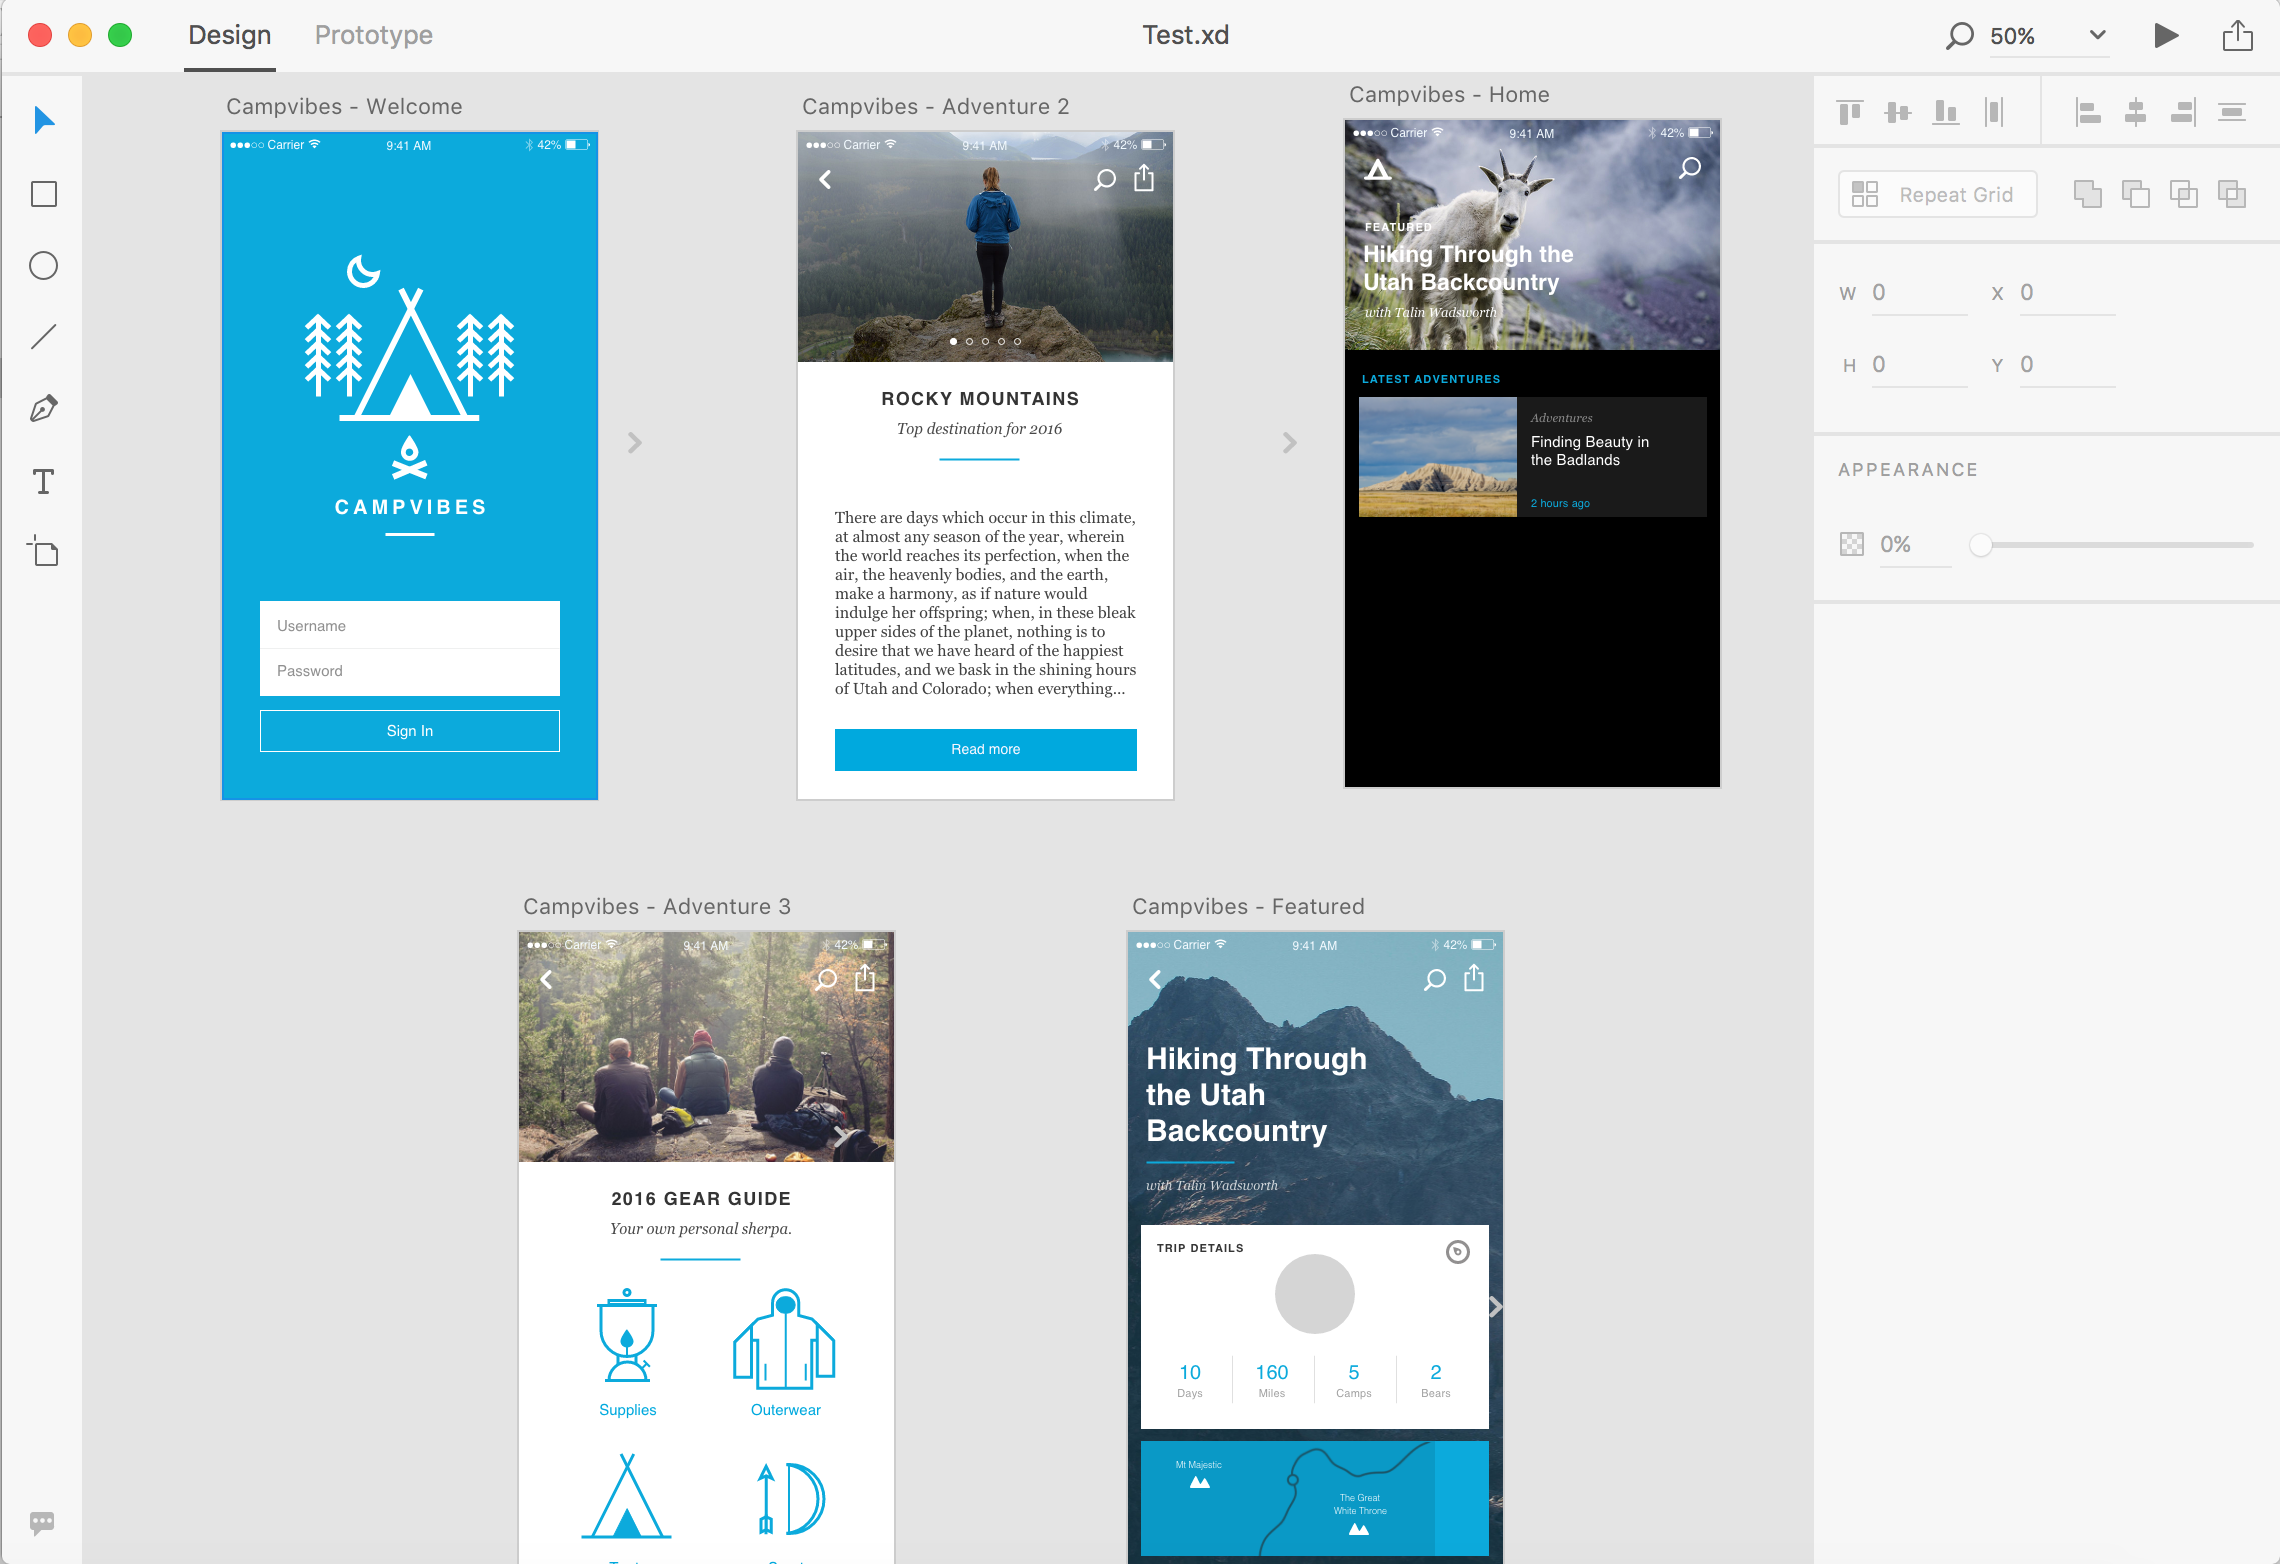
\includegraphics[width=.40\textwidth]{src/img/xdApp.png}};
\node (solutie) at (7, 0) {BlackBox Soluție};
\node (xcode) at (7, -5) {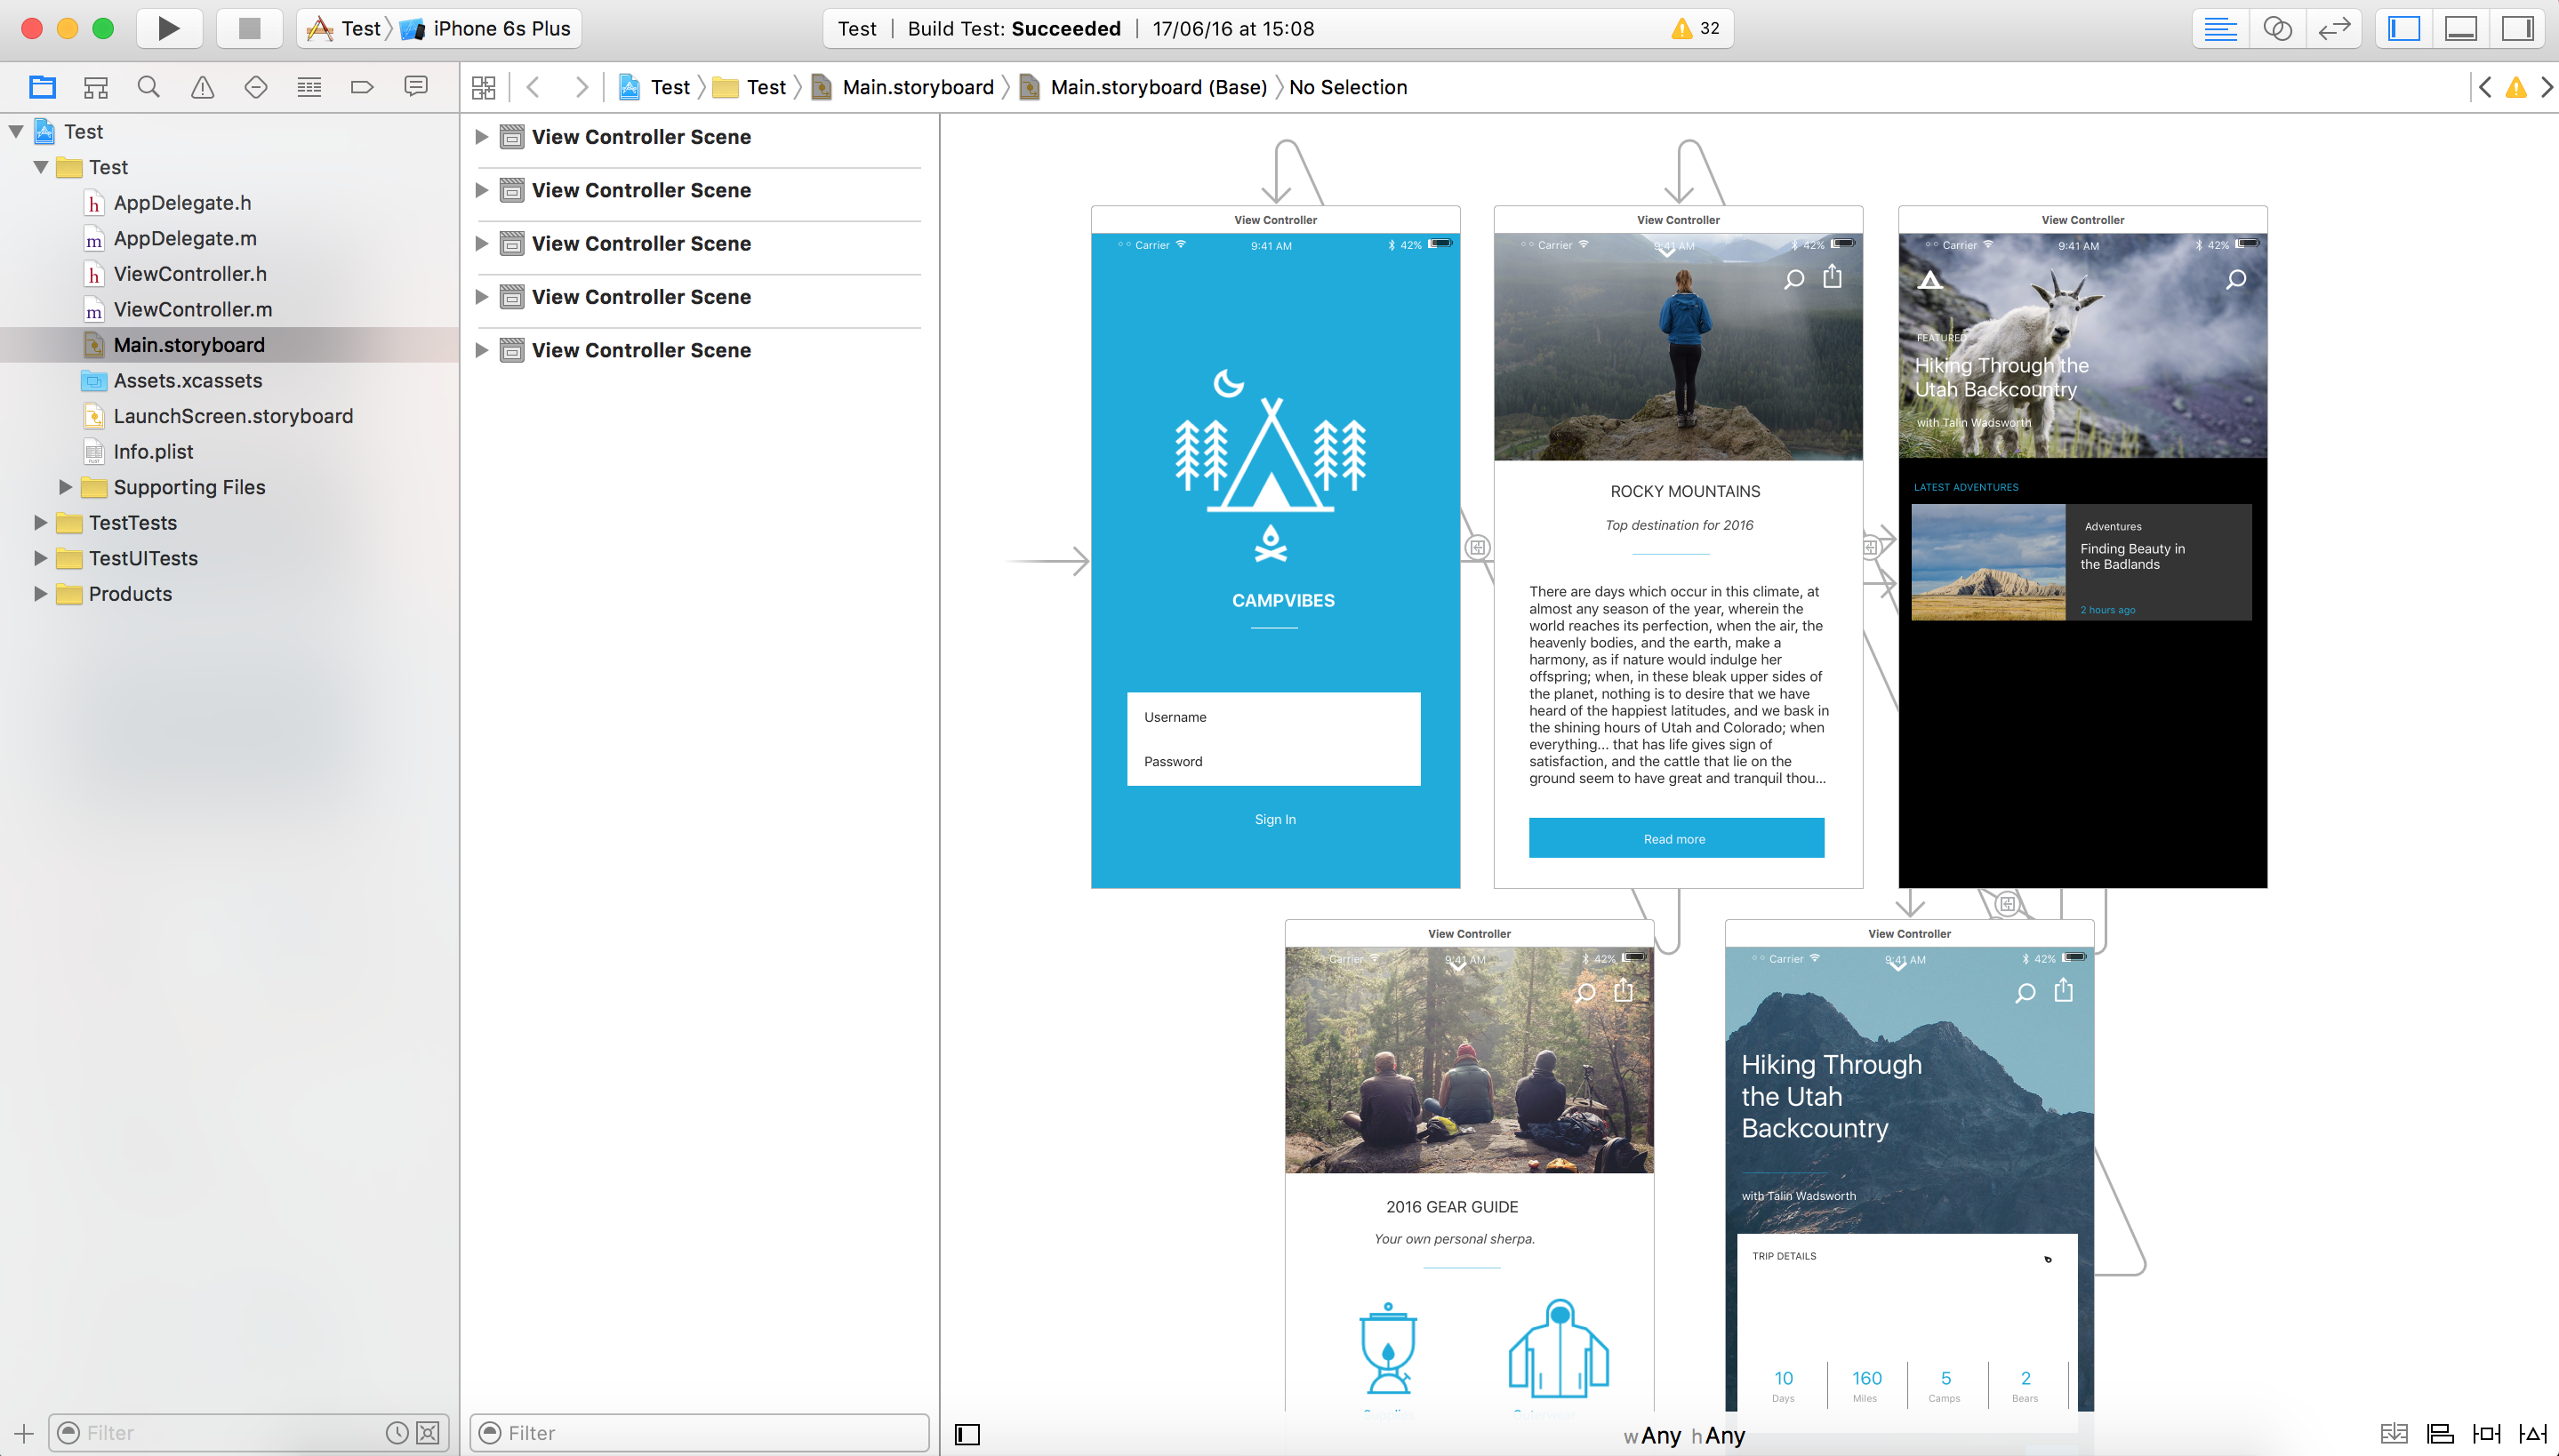
\includegraphics[width=.50\textwidth]{src/img/XcodeApp.png}};
\draw [<->](solutie) -- (xd);
\draw [<->] (xcode) -- (solutie);
\end{tikzpicture}
\caption{Flow-ul aplicației} \label{fig:Prezentare}
\end{figure}

Soluția prezentată (sau BlackBox-ul prezentat în figura \ref{fig:Prezentare}) se împarte într-o serie de module care implementează diferite concepte și funcționalități:
\begin{itemize} 
\item Xml2Dict: realizează translatarea din formatul xml corespunzător fișierului .storyboard într-un format json. SubTagurile corespunzătoare tagurilor $scene$ și $subviews$ vor fi transformate într-un vector de scene, respectiv de elemente vizuale.
\item Dict2Agc: primește ca input dicționarul json obținut de la modulul Xml2Dict și se folosește de o schemă de translatare XD - XCode (\ref{xcxd2schema}) pentru obținerea ierarhiei de fișiere xd;
\item XCode2XD: implementează funcționalitatea de translatare din reprezentarea XCode în reprezentarea XD (folosind prima schemă de translatare \ref{xcode2xdv1}); la baza acestui modul se află schema de translatare xml->json;
\item XD2XCode: implementează funcționalitatea de translatare din reprezentarea XD în reprezentarea XCode (\ref{xcxd2schema}); la baza acestui modul se află schema de translatare json->xml;
\item XDCreator: Creează ierarhia de fișiere .agc pentru construirea unui fișier de design xd (\ref{fig:ierarhie});
\item Sync: implementează funcționalitatea de sincronizare între XD și XCode(\ref{syncme}); monitorizează un fișier .xd, astfel încât orice modificare realizată în momentul salvării acestuia, să se revadă și în proiectul XCode asociat;
\item Helper: modul care implementează o serie de funcționalități generale necesare tuturor celorlalte module (ex. lucrul cu fișierele, crearea task-urilor pentru efectuarea de operații zip sau convert, etc.)
\end{itemize}

Aceste module și interacțiunea dintre ele este reprezentată în figura \ref{fig:Arhitectura}.

\begin{figure}[!htbp]
\centering
\begin{tikzpicture}[node distance = 4cm, auto]
\node [block] (xml2dict) {Xml2Dict};
\node [block, right of=xml2dict] (dict2agc) {Dict2Agc};
\node [block, right of=dict2agc] (xdcreator) {XDCreator};
\node [block, right of=xdcreator] (xd2xcode) {XD2XCode};
\node [block, below left=1cm and 1cm of xd2xcode] (sync) {Sync};
\node [block, below left=1cm and 1cm of xdcreator] (helper) {Helper};
\draw [->] (dict2agc) -- (xdcreator);
\draw [->] (sync) -- (xd2xcode);
\draw [->] (xml2dict) -- (dict2agc);
\draw [<->] (xml2dict) -- (helper);
\draw [<->] (dict2agc) -- (helper);
\draw [<->] (xdcreator) -- (helper);
\draw [<->] (sync) -- (helper);
\end{tikzpicture}
\caption{Arhitectură} \label{fig:Arhitectura}
\end{figure}

În arhitectura prezentată, modulul XCode2XD poate fi interschimbat cu modulele Xml2Dict și Dict2Agc, întrucât aceasta implementează aceeași funcționalitate, dar prin scheme de translatare diferite.

O tehnologie folosită pentru testarea și implementarea cu ajutorului Clipboardului este Clipboard Viewer \cite{clipboard}. Această aplicație arată conținutul oricărui clipboard, în funcție de tipul dorit. În cazul de față, pentru obținerea clipboardului specific aplicației Adobe XD, tipul clipboardului este reprezentat de ``com.adobe.sparkler.design".


\chapter{Performanțe}

În acest capitol voi prezenta o statistică a timpilor de rulare și voi compara schemele de translatare prezentate în capitolele anterioare (\ref{xcode2xdv1} și \ref{xcxd2schema}).

Schema de translatare este reprezentată într-un format .json din considerente de performanță. Un format json poate fi deserializat cu ușurință într-un dicționar imbricat, rezultând astfel o căutare rapidă a mapării dorite. Un astfel de dicționar asigură o complexitate de O(nn), unde nn reprezintă numărul de niveluri de imbricare ale dicționarului. În această aplicație numărul de niveluri nu depășește nn = 5.  

În continuare, voi prezenta graficele care specifică dependența dintre asset-uri ($Assets_processed$) și timpul de procesare al acestora ($Time_spent$) în funcție de schema de translatare aleasă.

\begin{figure}[!htbp]
\centering
    \begin{tikzpicture}
    \begin{axis}[
        xlabel=$Assets_processed$,
        ylabel=$Time_spent$]
    \addplot[smooth,mark=*,blue] plot coordinates {
        (51,0.004)
        (73,0.005)
        (95,0.009)
        (117,0.011)
        (160,0.025)
        (187,0.024)
        (231,0.027)
        (237,0.029)

    };
    \addlegendentry{Translatare Xml->Dictionar}
    \addplot[smooth,mark=*,red] plot coordinates {
        (51,0.26)
        (73,0.32)
        (95,0.47)
        (117, 0.52)
        (160, 0.64)
        (187,0.73)
        (231,0.83)
        (237,0.84)
    };
    \addlegendentry{Translatare Dictionar->Fișier XD}
    \end{axis}
    \end{tikzpicture}
\caption{Grafic XCode->XD (Schema Translatare 2)} \label{fig:Grafic1}
\end{figure}

\begin{figure}[!htbp]
\centering
\begin{tikzpicture}
    \begin{axis}[
        xlabel=$Assets_processed$,
        ylabel=$Time_spent$]
    \addplot[smooth,mark=*,blue] plot coordinates {
        (51,0.185)
        (73,0.189)
        (95,0.216)
        (117, 0.26)
        (160,0.32)
        (187,0.40)
        (231,0.55)
        (237,0.61)
    };
    \addlegendentry{Translatare XCode->XD}
    \end{axis}
    \end{tikzpicture}
\caption{Grafic XD->XCode (Schema Translatare 2)} \label{fig:Grafic1}
\end{figure}

Se poate observa faptul că cele două scheme de translatare XD - XCode, respectiv XCode - XD au timpi similari de rulare. Acest lucru era de așteptat având în vedere că implementările se bazează pe același model de schemă de translație. Un overhead se poate observa în cazul translatării din XCode în XD din cauza etapei intermediare de transformare a xml-ului într-un format json echivalent. De asemenea, în cazul translatării XCode - XD, apare o etapă computațională în plus față de translatarea XD - XCode. Această etapă constă în găsirea căii absolute ale imaginilor care se regăsesc în aplicația curentă. 

O primă variantă a aflării căii absolute ale acestor imagini a fost căutarea recursivă în directorul proiectului XCode, însă această abordare are două dezavantaje. În primul rând, există posibilitatea ca imaginile căutate să nu fie în directorul proiectului curent, iar în al doilea rând, așa cum se vede în figura \ref{fig:Tabimport} (coloana trei), timpii de căutare să fie mult mai mari decât timpul prpriu-zis de translatare. De aceea, se vor folosi informațiile din fișierul $project.pbxproj$. Acest fișier se poate regăsi în orice proiect de tipul XCode și va conține metadate legate de aplcația dezvoltată. Printre aceste metadate se află si informații cu privire la locația imaginilor folosite. Timpii de rulare pentru această metodă se regăsesc în tabelul \ref{fig:Tabimport} (coloana patru). Toți timpii de rulare din tabelul \ref{fig:Tabimport} sunt relativi la numărul de scene, respectiv numărul de proprietăți (coloanele cinci și șase). În prima coloană se specifică timpul de translatare dintr-un fișier xml (în cazul de față - storyboard-ul) într-un fișier json echivalent.

\begin{figure}[!htbp]
\centering
\begin{center}
    \begin{tabular}{| l | l | l | l |l |l |}
    \hline
    Nr. & Xml->Json & Json->Xd(V1) & Json->Xd(V2) & Nr Scene & Nr Proprietăți\\ \hline
    1 & 0.004 & 3.99 & 0.26 & 1 & 50\\ \hline
    2 & 0.005 & 4.96 & 0.32 & 2 & 73\\ \hline
    3 & 0.009 & 5.99 & 0.47 & 3 & 95\\ \hline
    4 & 0.011 & 7.05 & 0.52 & 4 & 117\\ \hline
    5 & 0.025 & 9.00 & 0.64 & 5 & 160\\ \hline
    6 & 0.026 & 10.60 & 0.73 & 5 & 187\\ \hline
    7 & 0.027 & 13.20 & 0.83 & 7 & 231\\ \hline
    \end{tabular}
\end{center}
\caption{Tabel Import} \label{fig:Tabimport}
\end{figure}

În figura \ref{fig:GraficSinc2} se pot observa diferențele dintre timpii de rulare a celor două metode de sincronizare. În graficul de culoare roșie se reprezintă sincronizarea XD - XCode prin generarea tuturor scenelor, independent de numărul de scene modificate. Graficul de culoare albastră specifică sincronizarea XD - XCode, dependentă de scenele modificate. Se poate observa o diferență semnificativă a timpilor de rulare în cazul în care un număr mic de scene vor fi modificate. Axa $X$ este reprezentată de numărul de scene modificate ($Modified_scenes$), iar axa $Y$ este reprezentată de timpul de rulare corespunzător metodei de sincronizare alese ($Time_spent$). Cele două grafice au fost generate pentru un număr de scene = 6.

\begin{figure}[!htbp]
\centering
\begin{tikzpicture}
    \begin{axis}[
        xlabel=$Modified_scenes$,
        ylabel=$Time_spent$]
    \addplot[smooth,color=blue,mark=x]
        plot coordinates {
            (1,0.11)
            (2,0.20)
            (3,0.26)
            (4,0.44)
        };
    \addlegendentry{Sincronizare V2}
    \addplot[smooth,color=red,mark=x]
        plot coordinates {
            (1,0.50)
            (2,0.50)
            (3,0.50)
            (4,0.50)
        };
    \addlegendentry{Sincronizare V1}
    
    \end{axis}
    \end{tikzpicture}
\caption{Grafic Sincronizare} \label{fig:GraficSinc2}
\end{figure}

\section{Comparație scheme de translatare}

După cum se observă în descrierea procedeelor de translatare XCode - XD(prima variantă - \ref{xcode2xdv1} )) și XD - XCode (\ref{xcxd2schema}), cele două scheme au metode de implementare destul de diferite. 

Prima schemă de translatare XCode - XD se bazează pe parcurgerea fișierului de input și pe realizarea translației pe măsură ce se procesează fișierul. Pentru ficare tag întâlnit se oferă un template care va fi procesat la rândul său pe baza regulilor definte. 

Există însă un dezavantaj major. Schema de translație XCode - XD nu poate afla categoria din care face parte un element vizual analizând numai tagul curent. De aceea, pe baza tagului părinte curent se va genera un template apoi, pe măsură ce se observă alte subtag-uri care indică faptul că tipul assetului curent este altul, se modifică și template-ul. Un exemplu al acestui caz este regăsit în cazul butoanelor. Un buton este reprezentat în figura \ref{fig:state}.

\begin{figure}[!htbp]
\lstset{language=XML}
\begin{lstlisting}
<button opaque="NO" ... id="qj4-Ou-Uog">
  <rect key="frame" x="68" y="189" width="212" height="120"/>
  <state key="normal" title="Button" image="art2.png"/>
</button>
\end{lstlisting}
\caption{Tipuri de butoane specificate prin tag-ul state} \label{fig:state}
\end{figure}

Tag-ul copil $state$ specifică faptul că butonul e fie de tip $text$, fie de tip $imagine$, în funcție de atributele prezente - $title$, respectiv $image$.

În momentul în care se ajunge la tag-ul $button$, se va construi un template json care specifică tipul - în mod default un buton de tip text. Dacă, însă, în momentul în care se ajunge la tag-ul copil $state$, iar atributul său corespuzător este $image$, template-ul trebuie înlocuit.

Acest neajuns este eliminat prin schema de translație XD - XCode. Această schemă asigură obținerea tipului corect de la începutul procesării datorită modului de obținere a tuturor caracteristicilor specifice unui element vizual. 
Așadar, în cazul de față, această schemă de translatare ar asigura găsirea corectă a tipului assetului prin verificarea tag-ului parinte și a atributelor specifice tag-ului $state$. De aceea, pentru a afla tipul corect al butonului - de tip text sau imagine, se verifică prezența atributelor $title$ sau $image$. În cazul în care apar ambele atribute în reprezentarea agc, vor fi construite două elemente vizuale - unul de tip text și altul de tip imagine. 

În principiu, neajunsul specificat în prima schemă de translatare este datorat tipului de fișier de intrare - xml - care permite procesarea unui singur tag la un moment dat. Complexitatea de procesare este de asemenea mai ridicată față de cea de-a doua schemă.
Schema de translatare folosită pentru conversia de la XD la XCode se poate folosi și în cazul translatării XCode - XD, prin conversia mai întâi a fișierului de input din xml în json (Această metodă a fost prezentată în detaliu în secțiunea \ref{xcxd2schema}).

O altă diferență majoră dintre cele două scheme de translatare ar fi ușurința de extindere, dar și de înțelegere. Schema de translatare XD - XCode asigură extensibilitate prin construirea template-ului, mapărilor și specificarea valorilor default într-o reprezentare ușoară și intuitivă. Specificarea unui comportament particularizat se poate construi prin adăugarea acestuia în cadrul schemei de translație și prin adăugarea unei funcții echivalente de implementare. 


\chapter{Concluzii}

În cadrul acestui proiect am prezentat o schemă de translatare dintre două aplicații de management al conținutului vizual pentru aplicații iOS - pe de o parte XCode, iar pe de altă parte Adobe Experience Design. Aceste scheme prezentate se pot extinde pentru translatarea formatelor care se pot serializa într-un dicționar (de ex. xml, json). De asemenea, s-a prezentat o soluție de sincronizare ale elementelor grafice între XD și XCode la nivel de scenă. Sincronizarea inversă se poate realiza în același mod prin implementarea algoritmului propus.

Această schemă de translatare se poate folosi în primul rând pentru managementul elementelor vizuale, așa cum este prezentată soluția de fața, dar se poate extinde pentru o serie de aplicații datorită schemei generale de translatare.

\section{Îmbunătățiri ulterioare}

Această aplicație se poate extinde ușor prin transformarea schemelor de translatare.
Câteva îmbunătățiri care se pot aduce acestei aplicații sunt:

\begin{enumerate}
\item Suport pentru multiple tipuri de controllere (Table View Controller, Collection View Controller, Navigation Controller, Tab Bar Controller, Page View Controller, GLKit View Controller sau Custom View Controller); Acest lucru se poate realiza prin extinderea schemei de translatare - definirea noilor mapări și dependențe;
\item Adăugare constrângeri pentru folosirea Auto Layout din cadrul Interface Builder;
\item Suport pentru multiple tipuri de interacțiuni (Show Detail etc.);
\item Translatarea multiplelor path-uri/figuri geometrice care aparțin aceluiași grup într-o singură imagine;
\item Reprezentarea vizuală a mapărilor - pentru extinderea facilă a aplicației;
\item Permiterea sincronizării pentru multiple fișiere; Acest lucru se va poate realiza prin modificarea ierarhiei de fișiere create în interiorul aplicției XCode;
\item Sincronizarea din XCode în XD - similar sincronizării inverse; Suport pentru apariția conflictelor de sincronizare (versionare);
\end{enumerate}


\begin{thebibliography}{9}
\bibitem{latexcompanion} 
XML Media Types, RFC 7303. Internet Engineering Task Force. July 2014.
 
\bibitem{einstein} 
Xcode on the Mac App Store. Apple Inc. Retrieved November 10, 2014
 
\bibitem{knuthwebsite} 
XML 1.0 Specification. World Wide Web Consortium. Retrieved 2010-08-22.

\bibitem{adobe}
Media Type Registration for image/svg+xml. W3C. Retrieved 5 February 2014 

\bibitem{svg}
Scalable Vector Graphics (SVG) 1.1 (Second Edition). W3C.

\bibitem{json}
ECMA-262 (ISO/IEC 16262), ECMAScript® Language Specification, 3rd edition (December 1999)

\bibitem{imageMagick}
http://www.imagemagick.org

\bibitem{clipboard}
https://developer.apple.com/library/mac/samplecode/ClipboardViewer/Introduction/Intro.html

\bibitem{repoGit}
https://github.com/ClaudiaRogoz/LicentaAdobe

\bibitem{lib}
https://developer.apple.com/library/mac/navigation/

\bibitem{xd}
http://www.adobe.com/products/experience-design.html

\bibitem{xcode}
https://developer.apple.com/xcode/

\bibitem{Aboutxcode}
https://en.wikipedia.org/wiki/Xcode

\bibitem{StructuraXcode}
http://fileformats.archiveteam.org/wiki/Xcode_Project
\end{thebibliography}

